%%%%%%%%%%%%%%%%%%%%%%%%%%%%%%%%%%%%%%%%%
%
% Template license:
% CC BY-NC-SA 3.0 (http://creativecommons.org/licenses/by-nc-sa/3.0/)
%
%%%%%%%%%%%%%%%%%%%%%%%%%%%%%%%%%%%%%%%%%

%----------------------------------------------------------------------------------------
%	PACKAGES AND OTHER DOCUMENT CONFIGURATIONS
%----------------------------------7------------------------------------------------------

\documentclass[
11pt, % The default document font size, options: 10pt, 11pt, 12pt
%oneside, % Two side (alternating margins) for binding by default, uncomment to switch to one side
%chapterinoneline,% Have the chapter title next to the number in one single line
spanish,
singlespacing, % Single line spacing, alternatives: onehalfspacing or doublespacing
%draft, % Uncomment to enable draft mode (no pictures, no links, overfull hboxes indicated)
%nolistspacing, % If the document is onehalfspacing or doublespacing, uncomment this to set spacing in lists to single
%liststotoc, % Uncomment to add the list of figures/tables/etc to the table of contents
%toctotoc, % Uncomment to add the main table of contents to the table of contents
parskip, % Uncomment to add space between paragraphs
%codirector, % Uncomment to add a codirector to the title page
headsepline, % Uncomment to get a line under the header
]{MastersDoctoralThesis} % The class file specifying the document structure
\usepackage{multirow}
\usepackage{verbatim} % comentarios

%----------------------------------------------------------------------------------------
%	INFORMACIÓN DE LA MEMORIA
%----------------------------------------------------------------------------------------

\thesistitle{Sistema de notificación de alarma de incendio} % El títulos de la memoria, se usa en la carátula y se puede usar el cualquier lugar del documento con el comando \ttitle

% Nombre del posgrado, se usa en la carátula y se puede usar el cualquier lugar del documento con el comando \degreename
\posgrado{Carrera de Especialización en Sistemas Embebidos} 
%\posgrado{Carrera de Especialización en Internet de las Cosas} 
%\posgrado{Carrera de Especialización en Intelegencia Artificial}
%\posgrado{Maestría en Sistemas Embebidos} 
%\posgrado{Maestría en Internet de las cosas}

\author{Ing. Daniel Marquez} % Tu nombre, se usa en la carátula y se puede usar el cualquier lugar del documento con el comando \authorname

\director{Mg. Ing. Wilmer Sanz (UC)} % El nombre del director, se usa en la carátula y se puede usar el cualquier lugar del documento con el comando \dirname
%\codirector{Nombre del Codirector (pertenencia)} % El nombre del codirector si lo hubiera, se usa en la carátula y se puede usar el cualquier lugar del documento con el comando \codirname.  Para activar este campo se debe descomentar la opción "codirector" en el comando \documentclass, línea 23.

\juradoUNO{Dr. Ing. Adrián Stacul (UTN, CITEDEF)} % Nombre y pertenencia del un jurado se usa en la carátula y se puede usar el cualquier lugar del documento con el comando \jur1name
\juradoDOS{Esp. Ing. Diego Fernández (FIUBA, DEBMEDIA)} % Nombre y pertenencia del un jurado se usa en la carátula y se puede usar el cualquier lugar del documento con el comando \jur2name
\juradoTRES{Esp. Ing. Santiago Salamandri (FIUBA)} % Nombre y pertenencia del un jurado se usa en la carátula y se puede usar el cualquier lugar del documento con el comando \jur3name

\fechaINICIO{marzo de 2020}
\fechaFINAL{diciembre de 2020}


\keywords{Sistemas Embebidos, FIUBA} % Keywords for your thesis, print it elsewhere with \keywordnames


\begin{document}


\frontmatter % Use roman page numbering style (i, ii, iii, iv...) for the pre-content pages

\pagestyle{plain} % Default to the plain heading style until the thesis style is called for the body content


%----------------------------------------------------------------------------------------
%	RESUMEN - ABSTRACT 
%----------------------------------------------------------------------------------------

\begin{abstract}
\addchaptertocentry{\abstractname} % Add the abstract to the table of contents
%
%The Thesis Abstract is written here (and usually kept to just this page). The page is kept centered vertically so can expand into the blank space above the title too\ldots
\centering

La presente memoria describe la implementación de un sistema de monitoreo de alarmas de incendio, con el objetivo de satisfacer la necesidad detectada por la firma Isolse SRL: brindar a sus clientes la posibilidad de conocer de forma remota el estado del sistema de detección de incendio.

El sistema se elabora utilizando conocimientos de programación de microcontroladores e ingeniería de software, protocolos de comunicación, diseño de circuitos impresos, manejo de bases de datos y micro-servidor web.

\end{abstract}

%----------------------------------------------------------------------------------------
%	CONTENIDO DE LA MEMORIA  - AGRADECIMIENTOS
%----------------------------------------------------------------------------------------

\begin{acknowledgements}
%\addchaptertocentry{\acknowledgementname} % Descomentando esta línea se puede agregar los agradecimientos al índice
\vspace{1.5cm}

Este trabajo es el resultado del esfuerzo de muchos. Aprovecho esta sección para agradecerles...

A Dios por la vida y la salud.

Mi familia por todo su apoyo y ánimo, el saber que están ahí para mí, me impulsa a mejorar y seguir creciendo cada día.   

Bettys Farias y Reinaldo Marquez, excelentes profesionales, amigos y mis queridos padres.

Andrea Fuenmayor, mi prometida con quien comparto este logro. Mi mejor amiga quien sin entender nada buscó todas las formas posibles para ayudarme.    

Marcos Ulloa, por su creatividad y compromiso. 

Ana Elisa, Marcela, Alicia, Hortencia, los Marcos y mis primos por siempre estar conmigo. No existe mayor inspiración que soñar con volver a verlos. 

A mi familia Argentina. Evelia, Julio, Mirta, Mariana, Rubén, Isabel quienes nos cuidaron y nos ayudaron a dar nuestros primeros pasos.  

Al equipo de la firma ISOLSE SRL, por todo su apoyo, confianza y la oportunidad de poder desarrollar el proyecto.

A todo el personal del Laboratorio de Sistema Embebidos de la FIUBA, por su enorme dedicación y excelencia. 

\end{acknowledgements}

%----------------------------------------------------------------------------------------
%	LISTA DE CONTENIDOS/FIGURAS/TABLAS
%----------------------------------------------------------------------------------------
\renewcommand{\listtablename}{Índice de Tablas} %TODO eliminar esta línea

\tableofcontents % Prints the main table of contents
%
\listoffigures % Prints the list of figures
%
\listoftables % Prints the list of tables


%----------------------------------------------------------------------------------------
%	CONTENIDO DE LA MEMORIA  - DEDICATORIA
%----------------------------------------------------------------------------------------

\dedicatory{
Este proyecto con todo el tiempo, esfuerzo y cariño que conllevó se lo dedico a mis hermanos Reinaldito, Alexander, Miguel, Felipe, Alejandro, Stephanie, Anabelle, Raúl, Víctor, José, Óscar y Oriana.

Que este trabajo los enorgullezca y los inspire a alcanzar sus metas, a soñar alto y a celebrar juntos todos nuestros logros. 


}  % escribir acá si se desea una dedicatoria

%----------------------------------------------------------------------------------------
%	CONTENIDO DE LA MEMORIA  - CAPÍTULOS
%----------------------------------------------------------------------------------------

\mainmatter % Begin numeric (1,2,3...) page numbering

\pagestyle{thesis} % Return the page headers back to the "thesis" style

%\renewcommand{\tablename}{Tabla} %TODO eliminar esta línea

% Incluir los capítulos como archivos separados desde la carpeta Chapters
% Descomentar las líneas a medida que se escriben los capítulos

% Chapter 1

\chapter{Introducción general} % Main chapter title

\label{Chapter1} % For referencing the chapter elsewhere, use \ref{Chapter1} 
\label{IntroGeneral}

%----------------------------------------------------------------------------------------

% Define some commands to keep the formatting separated from the content 
\newcommand{\keyword}[1]{\textbf{#1}}
\newcommand{\tabhead}[1]{\textbf{#1}}
\newcommand{\code}[1]{\texttt{#1}}
\newcommand{\file}[1]{\texttt{\bfseries#1}}
\newcommand{\option}[1]{\texttt{\itshape#1}}
\newcommand{\grados}{$^{\circ}$}

%----------------------------------------------------------------------------------------

%\section{Introducción}

%----------------------------------------------------------------------------------------

\chapter{Introducción específica} % Main chapter title

\label{Chapter2}

%----------------------------------------------------------------------------------------
%	SECTION 1
%----------------------------------------------------------------------------------------

En este capítulo se presentan los requerimientos del sistema y la planificación ejecutada. Además, se detallan las tecnologías utilizadas para el desarrollo tanto de software como de hardware del dispositivo primario y el dispositivo secundario.

\section{Detección de incendio}

Toda central de alarma de incendio debe notificar a los usuarios de la instalación de la presencia de un posible incidente y actuar en concordancia con el protocolo estipulado. Para ello generalmente el sistema segmenta los elementos de entrada y de salida según lo descrito en la figura \ref{fig:figura_a1}. Dividir el sistema facilita las conexiones, mantenimiento y respetar el estándar de la norma; en resumen la división consiste en: 

\begin{itemize}
\item  Lazo de detección: circuito eléctrico que contiene todos aquellos dispositivos asociados específicamente a la detección de posibles focos de incendio.
\item  Lazo de notificación: circuito eléctrico donde se encuentran aquellos equipos asociados a la notificación de un evento de alarma pueden ser parlantes, sirenas, luces estroboscópicas, entre otros.
\item  Interfaz con otros sistemas: relés programables ante diferentes eventos, un conjunto de interruptores que se utilizan para la notificación de eventos. Permite aislar el sistema y a la vez indicar de forma binaria el estado de un parámetro en particular.
\end{itemize}

\begin{figure}[h]
	\centering
	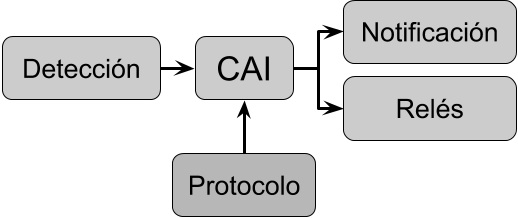
\includegraphics[scale=.45]{./Figures/Capitulo2/Figura_A.png}
	\caption{Diagrama de entradas y salidas de una central de alarma de incendio.}
	\label{fig:figura_a1}
\end{figure}

\section{Hardware}

Los componentes seleccionados para el sistema fueron seleccionados basados en los criterios de la sección \ref{criterios}. Existen tres componentes principales de hardware:  

\begin{itemize}
\item Raspberry Pi (dispositivo primario): es un computador de bajo costo que ejecuta un sistema operativo Linux \cite{RPI}. Tiene el tamaño de una tarjeta de crédito y cuenta con la capacidad de interactuar con componentes electrónicos externos mediante entradas y salidas de propósito general.

\begin{figure}[h]
	\centering
	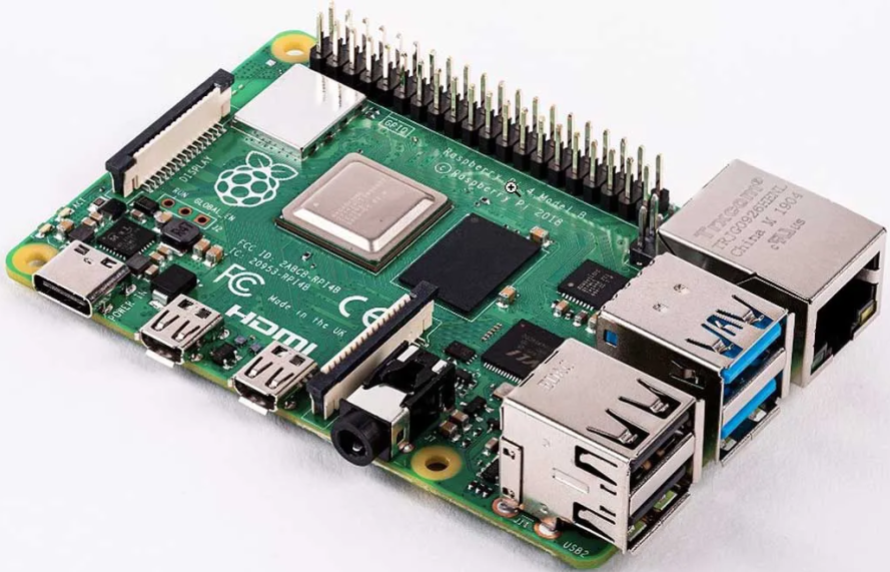
\includegraphics[scale=.25]{./Figures/Capitulo2/Figura_B.png}
	\caption{Raspberry Pi.}
	\label{fig:figura_b1}
\end{figure}


\item Node-MCU (dispositivo secundario): es un kit de desarrollo de bajo costo basado en el microcontrolador ESP8266 \cite{NODEMCU}. Algunas funcionalidades resaltantes son: regulador de tensión, entradas/salidas de propósito general y un  convertidor analógico digital. Permite el desarrollo de aplicaciones que requieren conexión a Internet de forma rápida, ya que incorpora conectividad Wi-Fi.

\begin{figure}[h]
	\centering
	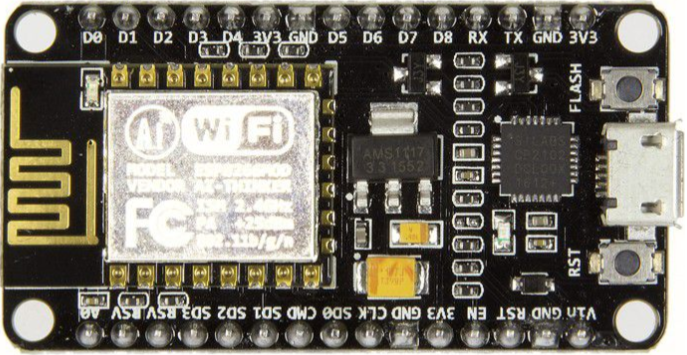
\includegraphics[scale=.25]{./Figures/Capitulo2/Figura_C.png}
	\caption{Node-MCU V3.0.}
	\label{fig:figura_c1}
\end{figure}

\item Nrf24l01 (comunicación inalámbrica): dispositivo transceptor \cite{rf24} con un protocolo incorporado de comunicación (Enhanced ShockBurst), que permite el diseño de sistemas comunicación inalámbrico con cualquier microcontrolador que cuente con comunicación SPI. Cuenta con parámetros configurables como frecuencia de trabajo (entre 2,400 - 2,4835 GHz), potencia y velocidad de transmisión de datos; lo que lo convierte en un sistema muy flexible para sistemas de bajo que requieran cumplir con requerimientos de bajo consumo.

\begin{figure}[h]
	\centering
	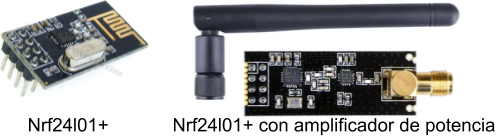
\includegraphics[scale=.65]{./Figures/Capitulo2/Figura_D.png}
	\caption{Nrf24l01+ y Nrf24l01+ con amplificador de potencia.}
	\label{fig:figura_d1}
\end{figure}
\end{itemize}

\section{Protocolos e interfaces}

Esta sección describe los protocolos que se utilizan internamente, junto con las plataformas y diferentes tecnologías empleadas por el sistema.      

\subsection{Protocolos de comunicación }
El sistema cuenta con diferentes equipos que se encuentran intercambiando información constantemente, por lo que se requiere de los siguientes protocolos que regulan la comunicación entre los dispositivos:

\begin{itemize}
\item  SPI (Serial Peripheral Interface): es un protocolo \cite{SPI} que permite la comunicación entre un dispositivo denominado “maestro” y varios dispositivos “esclavos”. El dispositivo maestro es responsable de iniciar la comunicación y define la tasa de transmisión basado en su señal de clock, es utilizado ampliamente entre microcontroladores y es el nexo que permite a los dispositivos primario y secundario interactuar con el transceptor Nrf24l01.

\item  TCP/IP + HTTP (Conexion a Internet ): el dispositivo primario requiere hacer la carga de información a un servidor web, para ello utiliza el protocolo TCP/IP para las capas de transporte y red, en conjunto con el protocolo HTTP para la capa de aplicación del estándar OSI.

\item  Enhanced Shockburst: un protocolo de comunicación basado en paquetes de datos que maneja de forma automática el empaquetado de la información, sincronización, transmisión y reconocimiento automático de transacciones. El protocolo soporta bidireccionalidad y se encuentra embebido en los elementos de la serie Nrf24lxx \cite{nrf24_protocol}.
\end{itemize}

\subsection{Interfaces}

El dispositivo primario otorga la información acerca del estado del sistema  al usuario. Requiere el desarrollo de Interfaces que permitan al usuario identificar fácilmente el estado de la instalación, al igual que un medio de acceso remoto sencillo que le permita acceder en cualquier momento.  

\begin{itemize}
\item Node-Red: herramienta de programación que provee una interfaz de desarrollo para servicios en línea \cite{node_red}. Funciona a través de programación en bloques y cuenta con diferentes integraciones con servicios de Internet, lo que facilita el desarrollo de interfaces de usuario personalizables.    

\item Firebase: es una plataforma de desarrollo de aplicaciones móviles \cite{firebase}. Brinda al usuario servicios de autenticación, bases de datos, almacenamiento, entre otros. Firebase permite realizar todas las conexiones necesarias para exportar la información desde el dispositivo primario a cualquier servicio de Internet, por ejemplo aplicaciones móviles o páginas web. 

\item Bases de datos con SQLite: SQLite es una biblioteca de funcionalidades reducidas que permite generar un motor de búsqueda SQL \cite{sqlite}. Las bases de datos generadas suelen utilizarse como contenedores de información para la transferencia organizada de información entre sistemas. EL uso de bases de datos permite registrar la información generada a partir de los análisis del dispositivo primario del sistema de detección de incendio.

\item MIT App Inventor: es un ambiente de programación en bloque que permite el diseño, simulación y construcción de aplicaciones para equipos móviles. Posee integración con Firebase por lo que con tan solo brindar los códigos de acceso, es posible acceder a la base de datos de cada proyecto.      
\end{itemize}

\section{Requerimientos}

A medida que se desarrollaba el sistema se realizaron reuniones mensuales con consultores y personal técnico de la empresa ISOLSE SRL. Los cambios más significativos consisten en facilitar el conexionado del sistema de monitoreo, eliminar la configuración manual y aprovechar los recursos del panel de control para el suministro eléctrico.   


\subsection{Normas de seguridad y garantía de servicio de Isolse SRL}
	\begin{enumerate}
	\item El sistema no deberá comprometer de ninguna manera el funcionamiento del sistema de detección de incendio.
	\item El sistema no deberá silenciar ni resetear los eventos presentes en el de detección de incendio de forma remota (basados en la norma NFPA punto 23.8.2.10 \cite{nfpa}). 
	\item El sistema de monitoreo remoto no transmitirá fallas internas al sistema de detección.
	\item El sistema de monitoreo deberá instalarse preferentemente en el mismo gabinete que la central de alarma.
	\end{enumerate}
	
\subsection{Funcionalidades comunes entre dispositivos primario y secundario}
	\begin{enumerate}
	\item Se realizará la adquisición del estado de los contactos secos.
		\begin{itemize}
		\item Contacto seco de falla en la central de alarma de incendio.
		\item Contacto seco de alarma en la central de alarma de incendio.
		\end{itemize}
	\item El suministro eléctrico deberá estar dentro del rango de los 12 a 24 VDC.
	\item Se deberá indicar el estado del sistema de detección de incendio a través de Leds, siguiendo la siguientes normas:
		\begin{itemize}
		\item  Verde en normal.
		\item  Amarillo para falla.
		\item  Rojo para alarma.
		\item   Rojo y amarillo para indicar alarma y falla presentes.				
		\end{itemize}
	\end{enumerate}
	
\subsection{Funcionalidades particulares del dispositivo primario}
	\begin{enumerate}
	\item Comunicación servidor web.
		\begin{enumerate}
		\item El sistema deberá tener la capacidad de transmitir información a un servidor web.
		\item La comunicación con el servidor web consistirá en enviar los siguientes datos al servidor web:
			\begin{itemize}
				\item La existencia de fallas en el sistema de detección de incendio. 	
				\item La existencia de alarmas en el sistema de detección de incendio.
				\item La presencia de fallas en el sistema de comunicación inalámbrica.
			\end{itemize}
		\item Se deberá establecer una comunicación con el servidor, ante un evento de cambio de estado del sistema de detección, en un intervalo de tiempo menor a 10 segundos.
		\item Se establecerá una comunicación inmediata con servidor web, si ocurre un cambio en el estado de los contactos secos.
		\item Se deberá establecer una comunicación con el servidor, ante un evento cambio de estado del sistema de comunicación inalámbrica, en un intervalo de tiempo menor a 10 segundos.
		\item Se generará un software encargado de generar y transmitir los paquetes de datos JSON.
		\item Se deberá establecer una prueba que permita verificar el funcionamiento de la comunicación con el servidor web. 
		\end{enumerate}
	\item Se registrarán al menos 500 eventos de forma local.
	\item Comunicación inalámbrica.
		\begin{enumerate}		
		\item Se realizará la adquisición del estado de los dispositivos secundarios a partir de los contactos secos monitoreados:
			\begin{itemize}
				\item Contacto seco de falla en la central de alarma de incendio.
				\item Contacto seco de alarma en la central de alarma de incendio.
			\end{itemize}	
		\item Se debe diseñar un mecanismo de recuperación ante fallas de comunicación inalámbrica.	
		\item Se realizará un software con la capacidad de recibir información por radiofrecuencia con hasta 3 dispositivos secundarios.
		\item Se establecerá una comunicación periódica con todos los dispositivos secundarios con una tasa de refresco de  al menos cada 2,5 s.
		\item Se deberá crear un software para controlar la secuencia de comunicación con dispositivos secundarios.
		\item Se deberá procesar los datos provenientes de dispositivos secundarios, para determinar los estados reales de la instalación.
		\item Se deberá establecer una prueba que permita verificar el funcionamiento de la comunicación por radiofrecuencia.
	\end{enumerate}
\end{enumerate}
\subsection{Funcionalidades particulares del dispositivo secundario}
	\begin{enumerate}	
		\item Se realizará un software con la capacidad de transmitir información por radiofrecuencia al dispositivo primario.
		\item Se establecerá una comunicación periódica con el dispositivo primario con una tasa de refresco de al menos cada 2,5 s.
		\item Se implementará un software con capacidad de reinicio, ante un total de 150 o más intentos fallidos de comunicación inalámbrica.
		\item Se deberá establecer una prueba que permita verificar el funcionamiento de la comunicación inalámbrica.
	\end{enumerate}
	
\subsection{Condiciones de trabajo}
	\begin{enumerate}
		\item Idealmente el sistema tendrá que estar resguardado dentro de la central de incendio, en caso contrario se requerirá una protección IP51.
	\end{enumerate}


\begin{comment}
\begin{enumerate}
\item Normas de seguridad y garantía de servicio de Isolse SRL.
	\begin{enumerate}
	\item El sistema no deberá comprometer de ninguna manera el funcionamiento del sistema de detección de incendio.
	\item El sistema no deberá silenciar ni resetear los eventos presentes en el de detección de incendio de forma remota. 
	\item El sistema de monitoreo remoto no transmitirá fallas internas al sistema de detección.
	\item En caso de corte del suministro eléctrico el sistema no deberá afectar de ninguna manera la autonomía de la central.
	\item El sistema de monitoreo deberá instalarse preferentemente en el mismo gabinete que la central de alarma.
	\end{enumerate}
\item Funcionalidades comunes entre dispositivos primario y secundario.
	\begin{enumerate}
	\item Se realizará la adquisición del estado de los contactos secos.
		\begin{itemize}
		\item Contacto seco de falla en la central de alarma de incendio.
		\item Contacto seco de alarma en la central de alarma de incendio.
		\end{itemize}
	\item El suministro eléctrico deberá estar dentro del rango de los 12 a 24 VDC.
	\item Se deberá indicar el estado del sistema de detección de incendio a través de Leds, siguiendo la siguientes normas:
		\begin{itemize}
		\item  Verde en normal.
		\item  Amarillo para falla.
		\item  Rojo para alarma.
		\item   Rojo y amarillo para indicar alarma y falla presentes.				
		\end{itemize}
	\end{enumerate}
\item Funcionalidades particulares del dispositivo primario.
	\begin{enumerate}
	\item Comunicación servidor web.
		\begin{enumerate}
		\item El sistema deberá tener la capacidad de transmitir información a un servidor web.
		\item La comunicación con el servidor web consistirá en enviar los siguientes datos al servidor web:
			\begin{itemize}
				\item La existencia de fallas en el sistema de detección de incendio. 	
				\item La existencia de alarmas en el sistema de detección de incendio.
				\item La presencia de fallas en el sistema de comunicación inalámbrica.
			\end{itemize}
		\item Se deberá establecer una comunicación con el servidor, ante un evento de cambio de estado del sistema de detección, en un intervalo de tiempo menor a 10 segundos.
		\item Se establecerá una comunicación inmediata con servidor web, si ocurre un cambio en el estado de los contactos secos.
		\item Se deberá establecer una comunicación con el servidor, ante un evento cambio de estado del sistema de comunicación inalámbrica, en un intervalo de tiempo menor a 10 segundos.
		\item Se generará un software encargado de generar y transmitir los paquetes de datos JSON.
		\item Se deberá establecer una prueba que permita verificar el funcionamiento de la comunicación con el servidor web. 
		\end{enumerate}
	\item Se registrarán al menos 500 eventos de forma local.
	\item Comunicación inalámbrica.
		\begin{enumerate}		
		\item Se realizará la adquisición del estado de los dispositivos secundarios a partir de los contactos secos monitoreados:
			\begin{itemize}
				\item Contacto seco de falla en la central de alarma de incendio.
				\item Contacto seco de alarma en la central de alarma de incendio.
			\end{itemize}	
		\item Se debe diseñar un mecanismo de recuperación ante fallas de comunicación inalámbrica.	
		\item Se realizará un software con la capacidad de recibir información por radiofrecuencia con hasta 3 dispositivos secundarios.
		\item Se establecerá una comunicación periódica con todos los dispositivos secundarios con una tasa de refresco de  al menos cada 2,5 s.
		\item Se deberá crear un software para controlar la secuencia de comunicación con dispositivos secundarios.
		\item Se deberá procesar los datos provenientes de dispositivos secundarios, para determinar los estados reales de la instalación.
		\item Se deberá establecer una prueba que permita verificar el funcionamiento de la comunicación por radiofrecuencia.
	\end{enumerate}
\end{enumerate}
\item Funcionalidades particulares del dispositivo secundario.
	\begin{enumerate}	
		\item Se realizará un software con la capacidad de transmitir información por radiofrecuencia al dispositivo primario.
		\item Se establecerá una comunicación periódica con el dispositivo primario con una tasa de refresco de al menos cada 2,5 s.
		\item Se implementará un software con capacidad de reinicio, ante un total de 150 o más intentos fallidos de comunicación inalámbrica.
		\item Se deberá establecer una prueba que permita verificar el funcionamiento de la comunicación inalámbrica.
	\end{enumerate}
\item Condiciones de trabajo.
	\begin{enumerate}
		\item Idealmente el sistema tendrá que estar resguardado dentro de la central de incendio, en caso contrario se requerirá una protección IP51.
	\end{enumerate}
\end{enumerate}
\end{comment}
 
%\subsection{Uso del Nrf24l01+}
%\begin{itemize}
%\item  Nrf24l01 amplificador de potencia con reducción de ruido y antena.
%\item  Nrf24l01 + anten
%\item  Fuente de poder Canakit micro USB 2,5 A con filtro de ruido.
%\item Adaptador 120-240 VA a 5V DC USB.
%\end{itemize}

%\begin{figure}[ht]
%	\centering
%	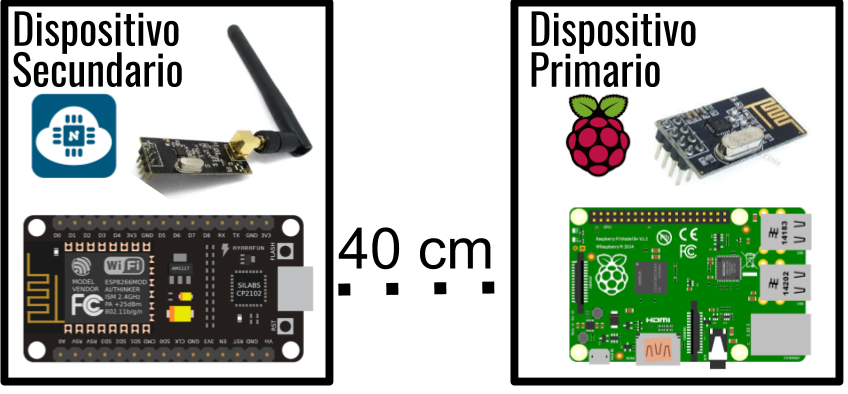
\includegraphics[scale=.45]{./Figures/Capitulo4/Figura_A.png}
%	\caption{Esquema utilizado para el ensayo del Nrf24l01+.}
%	\label{fig:figura_a}
%\end{figure}
%\ref{fig:figura_a}
 
\chapter{Diseño e implementación} % Main chapter title

\label{Chapter3} % Change X to a consecutive number; for referencing this chapter elsewhere, use \ref{ChapterX}

\definecolor{mygreen}{rgb}{0,0.6,0}
\definecolor{mygray}{rgb}{0.5,0.5,0.5}
\definecolor{mymauve}{rgb}{0.58,0,0.82}

%%%%%%%%%%%%%%%%%%%%%%%%%%%%%%%%%%%%%%%%%%%%%%%%%%%%%%%%%%%%%%%%%%%%%%%%%%%%%
% parámetros para configurar el formato del código en los entornos lstlisting
%%%%%%%%%%%%%%%%%%%%%%%%%%%%%%%%%%%%%%%%%%%%%%%%%%%%%%%%%%%%%%%%%%%%%%%%%%%%%
\lstset{ %
  backgroundcolor=\color{white},   % choose the background color; you must add \usepackage{color} or \usepackage{xcolor}
  basicstyle=\footnotesize,        % the size of the fonts that are used for the code
  breakatwhitespace=false,         % sets if automatic breaks should only happen at whitespace
  breaklines=true,                 % sets automatic line breaking
  captionpos=b,                    % sets the caption-position to bottom
  commentstyle=\color{mygreen},    % comment style
  deletekeywords={...},            % if you want to delete keywords from the given language
  %escapeinside={\%*}{*)},          % if you want to add LaTeX within your code
  %extendedchars=true,              % lets you use non-ASCII characters; for 8-bits encodings only, does not work with UTF-8
  %frame=single,	                % adds a frame around the code
  keepspaces=true,                 % keeps spaces in text, useful for keeping indentation of code (possibly needs columns=flexible)
  keywordstyle=\color{blue},       % keyword style
  language=[ANSI]C,                % the language of the code
  %otherkeywords={*,...},           % if you want to add more keywords to the set
  numbers=left,                    % where to put the line-numbers; possible values are (none, left, right)
  numbersep=5pt,                   % how far the line-numbers are from the code
  numberstyle=\tiny\color{mygray}, % the style that is used for the line-numbers
  rulecolor=\color{black},         % if not set, the frame-color may be changed on line-breaks within not-black text (e.g. comments (green here))
  showspaces=false,                % show spaces everywhere adding particular underscores; it overrides 'showstringspaces'
  showstringspaces=false,          % underline spaces within strings only
  showtabs=false,                  % show tabs within strings adding particular underscores
  stepnumber=1,                    % the step between two line-numbers. If it's 1, each line will be numbered
  stringstyle=\color{mymauve},     % string literal style
  tabsize=2,	                   % sets default tabsize to 2 spaces
  title=\lstname,                  % show the filename of files included with \lstinputlisting; also try caption instead of title
  morecomment=[s]{/*}{*/}
}


%----------------------------------------------------------------------------------------
%	SECTION 1
%----------------------------------------------------------------------------------------

En este capítulo se exponen los detalles del diseño de los dispositivos primario y secundario, se describe el desarrollo y funcionamiento del hardware, software y las características más resaltantes del proyecto.

\section{Sistemas complejos de detección de incendio}

Un sistema de detección de incendio no se limita necesariamente a un solo edificio. En instalaciones de mayor escala conformadas por varias infraestructuras ya sean industriales o residenciales, es común utilizar sistemas complejos de detección de incendio. También se utilizan en áreas como depósitos de materiales, salas de máquinas o cuartos de generadores eléctricos de respaldo, y en cuartos con tanques de almacenamiento de agua para sistemas de bombeo de extinción de incendios.

En este nivel los sistemas suelen estar compuestos por más de una central de alarma de incendio, que pueden estar interconectadas entre sí y formar una red de dispositivos de detección. Dependiendo del nivel de integración, los sistemas pueden tener total independencia o por el contrario funcionar como una única unidad de detección, por lo que  no siempre es una tarea sencilla identificar la ubicación de origen de un evento.

Un ejemplo de una instalación con potencial para un sistema de detección de incendio complejo puede observarse en la figura \ref{fig:figura_a3}, se puede apreciar una propiedad compuesta por tres edificios y una zona crítica, con una posible estructura de dispositivos primarios y secundarios que permite definir el estado del sistema de detección de incendio en su totalidad.


\begin{figure}[]
	\centering
	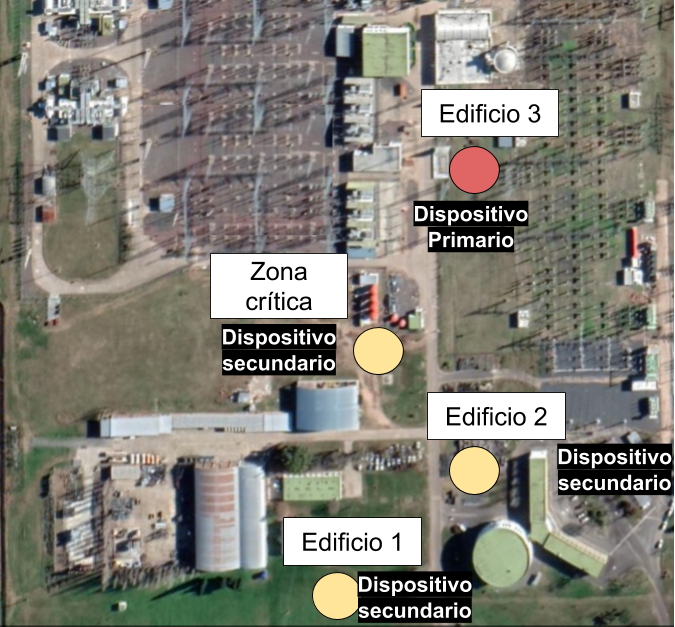
\includegraphics[scale=.4]{./Figures/Capitulo3/Fig_A3.png}
	\caption{Ejemplo de sistema de detección de incendio complejo.}
	\label{fig:figura_a3}
\end{figure}

\section{Criterios de diseño}

El sistema corresponde al primero de una serie de proyectos que tienen como objetivo la generación de alternativas de monitoreo de sistemas de detección de incendio. En esta etapa el objetivo propuesto es reportar al usuario únicamente el estado de la instalación, pero en futuros proyectos se desea alcanzar un mayor nivel de detalle. A continuación se describen los criterios considerados para la selección de los componentes:

Escalabilidad: el sistema debe contar con los recursos necesarios para la integración de nuevas funcionalidades o servicios.

Robustez: una característica que se desea proporcionar a los sistemas es la posibilidad de tener formas alternativas de trabajo ante eventos de falla.

Recuperabilidad: el mantenimiento de equipos de detección de incendio suele realizarse de forma mensual, por lo que el sistema debe estar en capacidad de restituirse de forma automática en caso de fallas, para evitar visitas adicionales por fallas del dispositivo de monitoreo.

Documentación adecuada:  el sistema debe desarrollarse a partir de plataformas con documentación detallada y de fácil acceso.

Disponibilidad en el mercado argentino: los sistemas deberán estar compuestos por elementos que puedan ser adquiridos en el mercado local.

\subsubsection{Criterios fundamentales}

Es de suma importancia respetar dos criterios principales:
\begin{itemize}
\item La no afectación la secuencia de accionamiento de la central de forma remota. 
\item El sistema de monitoreo no debe utilizarse como un dispositivo de detección de incendio.
\end{itemize}

El esquema de conexión entre el dispositivo de monitoreo y la central de alarma de incendio recomendado
se muestra en la figura \ref{fig:figura_b3}.

\begin{figure}[]
	\centering
	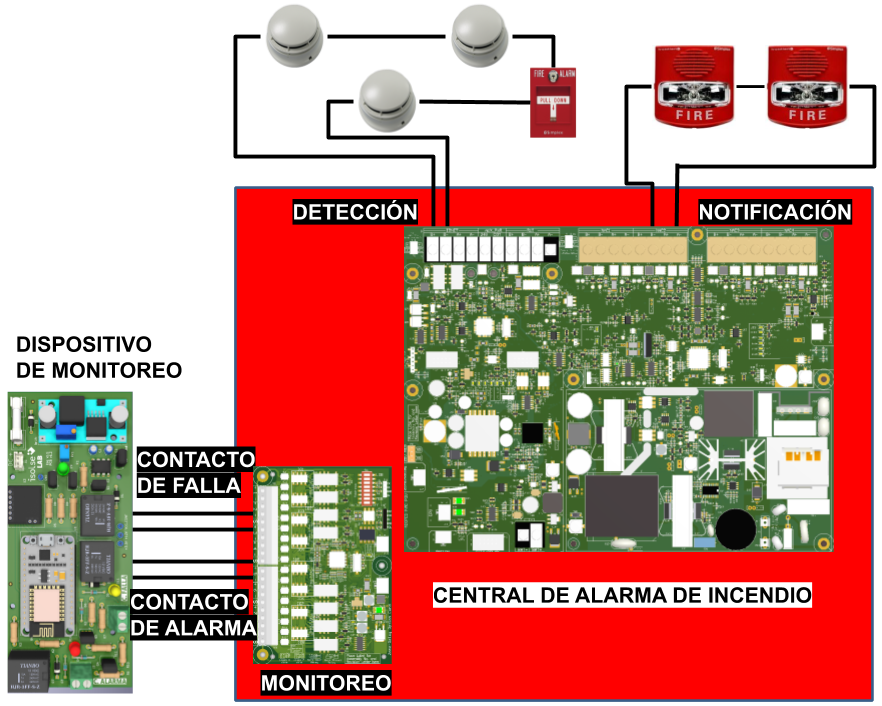
\includegraphics[scale=.35]{./Figures/Capitulo3/Fig_B3.png}
	\caption{Esquema de conexión entre dispositivo de monitoreo y central de alarma de incendio.}
	\label{fig:figura_b3}
\end{figure}

\section{Arquitectura general del sistema}

En esta fase se procede a describir los elementos que componen el sistema de monitoreo, su funcionamiento y la interconexión entre cada componente.


\subsection{Dispositivo primario} 

Un sistema de monitoreo compuesto por este dispositivo únicamente cuenta con los recursos necesarios para el monitoreo de un sistema de detección de alarma base, compuesto por una única central de alarma de incendio a monitorear. El dispositivo implementa un monitoreo periodico a los contactos de alarma y falla para determinar el estado del equipo local; el siguiente paso es facilitar esta información al usuario  para lo que hace uso de tres recursos de notificación:
\begin{itemize}
\item Leds de indicación de estado.
\item Interfaz web para notificación local, por medio de la plataforma Node-RED.
\item Servidor web firebase.
\end{itemize}

A pesar de ser un dispositivo para el monitoreo de un sistema de detección de alarma base este dispositivo considera la posibilidad de un sistema de detección complejo, por lo que dispone de un módulo específico para la gestión de comunicación inalámbrica que permite al sistema comunicarse con diferentes dispositivos de monitoreo secundarios.

El dispositivo primario procesa el estado local y los estados remotos para generar un diagnóstico del sistema de detección en general, de esta forma en caso de no existir vinculación entre los equipos de detección de alarma el sistema es capaz de establecer el estado correcto de la instalación en su totalidad.

El diseño general del dispositivo primario se puede observar en la figura \ref{fig:figura_c3}.

\begin{figure}[h]
	\centering
	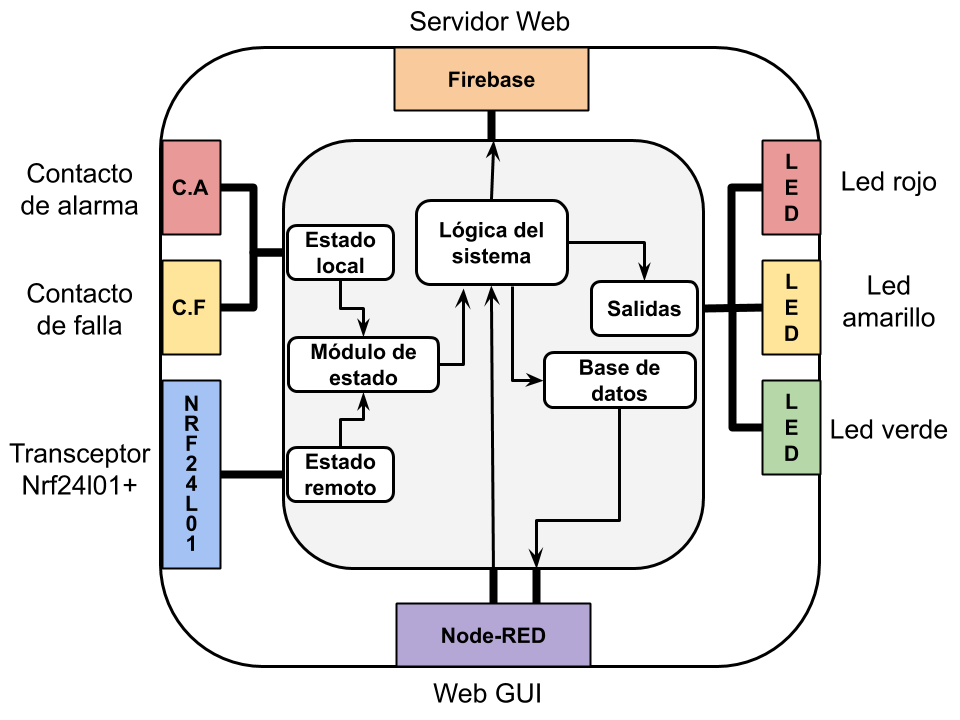
\includegraphics[scale=.4]{./Figures/Capitulo3/Fig_C3.png}
	\caption{Arquitectura del dispositivo primario.}
	\label{fig:figura_c3}
\end{figure}

\subsection{Dispositivo secundario}

Este dispositivo realiza el  monitoreo del contacto de alarma y del contacto de falla, y cuenta con módulo destinado a la gestión de la transmisión de información mediante comunicación inalámbrica. El sistema presenta la información al usuario de acuerdo a la condición existente en la instalación: rojo indica alarma, amarillo indica falla y verde, condición normal.


Incluir en el diseño un dispositivo secundario permite agregar un equipo adicional a monitorear, y además incrementa el alcance de la comunicación inalámbrica, ya que cada nodo actúa como nodo-repetidor. En la figura \ref{fig:figura_d3} se observa el diseño general del dispositivo secundario.


\begin{figure}[]
	\centering
	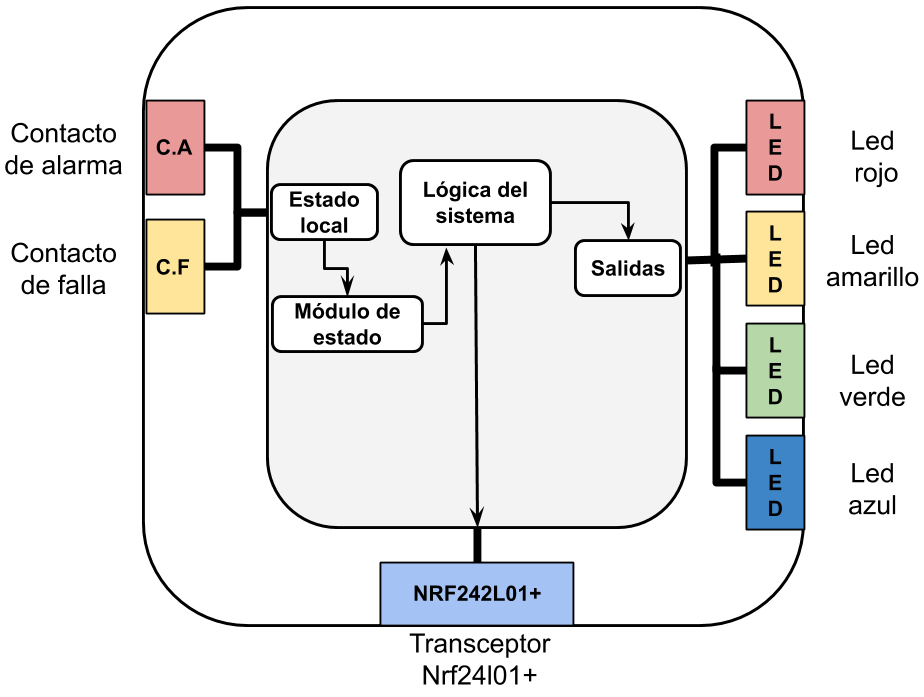
\includegraphics[scale=.4]{./Figures/Capitulo3/Fig_D3.png}
	\caption{Arquitectura del dispositivo secundario.}
	\label{fig:figura_d3}
\end{figure} 

\subsection{Aplicación en sistemas de detección complejos}

Una instalación como la descrita en la figura \ref{fig:figura_a3}, compuesta por tres edificios y una zona crítica, puede ser monitoreada con una arquitectura como la dispuesta en la figura \ref{fig:figura_e3}, donde se puede observar las interfaces entre los elementos del sistema.

\begin{figure}[]
	\centering
	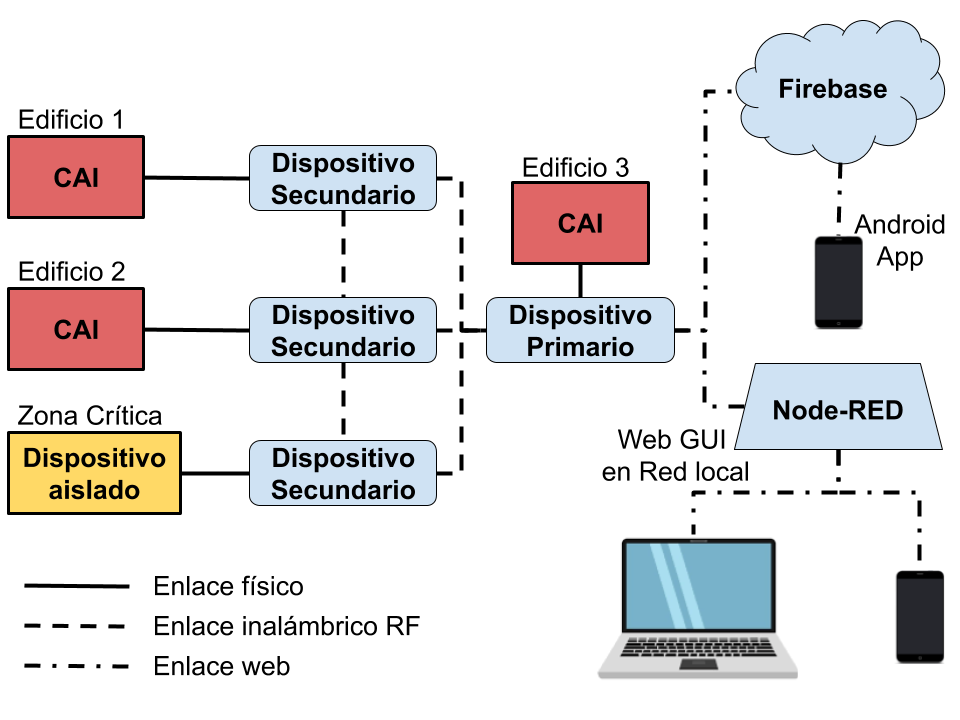
\includegraphics[scale=.4]{./Figures/Capitulo3/Fig_E3.png}
	\caption{Arquitectura general del dispositivo de monitoreo remoto.}
	\label{fig:figura_e3}
\end{figure} 

\newpage

\section{Hardware}

Esta sección describe el  diseño del hardware utilizado para los dispositivos primario y secundario, sus características, módulos internos y la relación entre ellos.

\subsection{Hardware del dispositivo primario}

Los esquemáticos empleados para la implementación del hardware del dispositivo primario se pueden observar en las figuras \ref{fig:figura_f3}, \ref{fig:figura_g3} y \ref{fig:figura_h3}. El diseño fue concretado como un poncho para la Raspberry Pi, compuesto por los módulos detallados a continuación:

\subsubsection{Módulo de monitoreo de contacto seco}

El diseño de este módulo hace uso del contacto normal abierto del dispositivo a monitorear para la indicación de alarma o falla en el sistema. La indicación correspondiente se hace a través del accionamiento de un relé interno que modifica el estado del circuito asociado.
La figura \ref{fig:figura_f3} muestra el esquema del módulo de monitoreo de contacto seco.

\begin{figure}[]
	\centering
	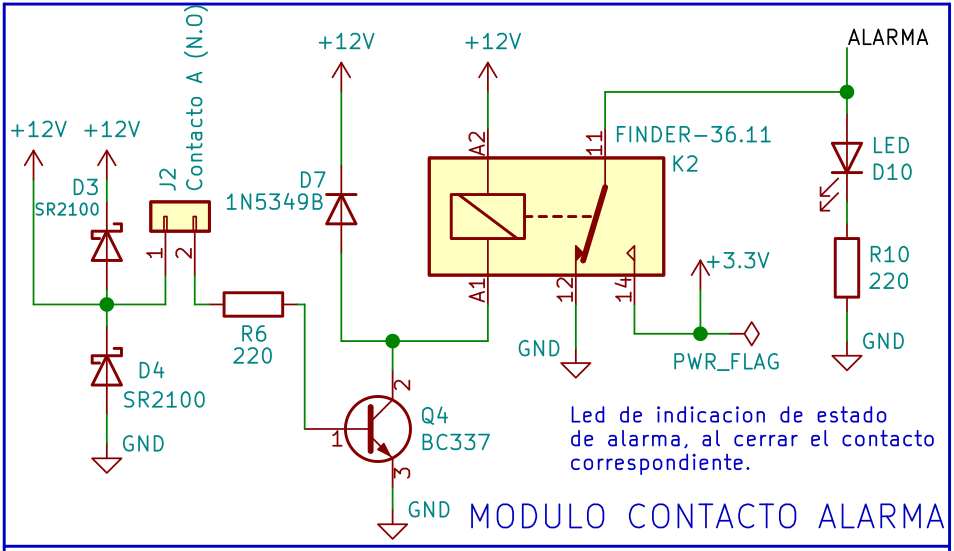
\includegraphics[scale=.35]{./Figures/Capitulo3/Fig_F3.png}
	\caption{Módulo de monitoreo de contacto seco de alarma.}
	\label{fig:figura_f3}
\end{figure} 

El diseño considera la posibilidad de ocurrencia de un error de conexión, para lo cual se incluyó una etapa de protección, que se encarga de mantener la tensión dentro de los rangos de trabajo del dispositivo [0 - 12] VDC.

\subsubsection{Módulo de comunicación nrf24l01+}

La conexión del módulo transceptor nrf24l01+ se hace siguiendo el esquema recomendado [bibliografía], como puede observarse en la figura \ref{fig:figura_g3}, consiste en una conexión directa con el dispositivo y en utilizar la fuente de 3,3 VDC del dispositivo primaria para energizarlo.  

\begin{figure}[]
	\centering
	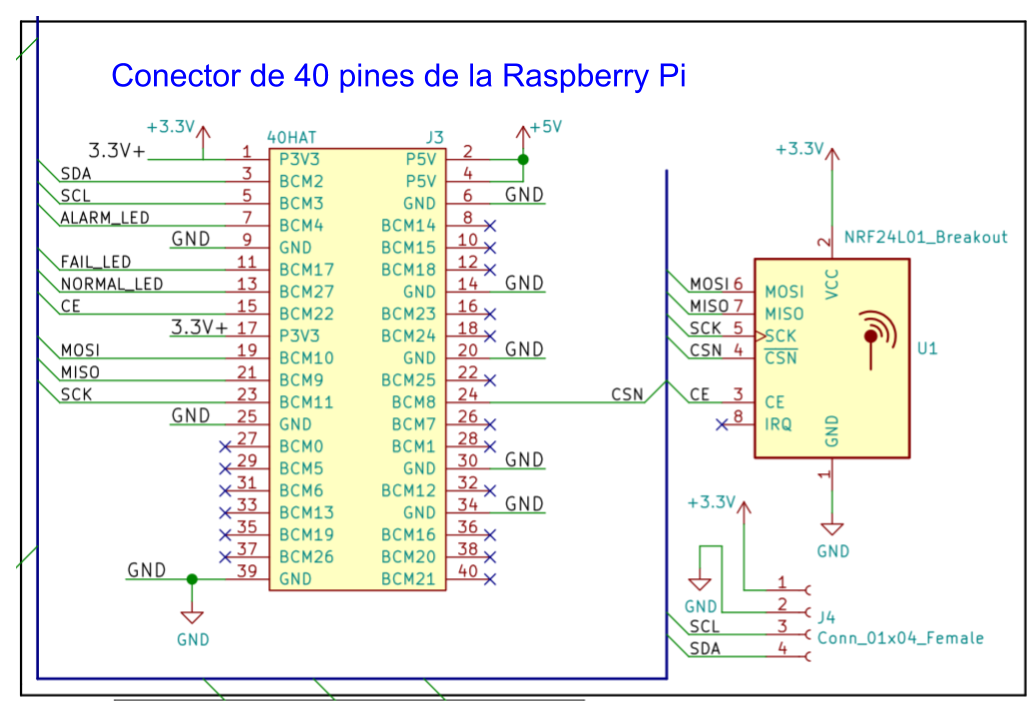
\includegraphics[scale=.35]{./Figures/Capitulo3/Fig_G3.png}
	\caption{Módulo de comunicación inalámbrica.}
	\label{fig:figura_g3}
\end{figure} 

\subsubsection{Módulo de notificación visual}

El módulo sigue lo establecido por los requerimientos  2.3.9 y permite al dispositivo reportar el estado del sistema a monitorear de forma local, sin necesidad de dispositivos adicionales. En la figura \ref{fig:figura_h3} se presentan las conexiones y pines utilizados por el sistema.

\begin{figure}[]
	\centering
	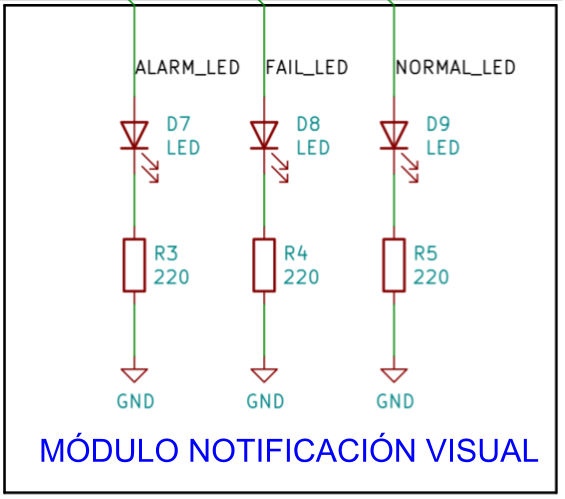
\includegraphics[scale=.25]{./Figures/Capitulo3/Fig_H3.png}
	\caption{Módulo de notificación visual.}
	\label{fig:figura_h3}
\end{figure} 


\subsection{Hardware del dispositivo secundario}

El diseño del sistema puede observarse en las figuras \ref{fig:figura_j3},\ref{fig:figura_k3},\ref{fig:figura_l3}, se reutiliza el diseño de la figura \ref{fig:figura_f3} para el monitoreo de contactos y se añaden al sistema los módulos descritos a continuación.

\subsubsection{Módulo de comunicación nrf24l01+ con amplificador de potencia}

El dispositivo secundario utiliza un módulo nrf24l01+ con un amplificador de potencia, por lo que a diferencia del dispositivo primario emplea un adaptador para la conexión del módulo que garantiza una tensión de alimentación estable. El esquema de conexión se detalla en la figura \ref{fig:figura_j3}.

\begin{figure}[]
	\centering
	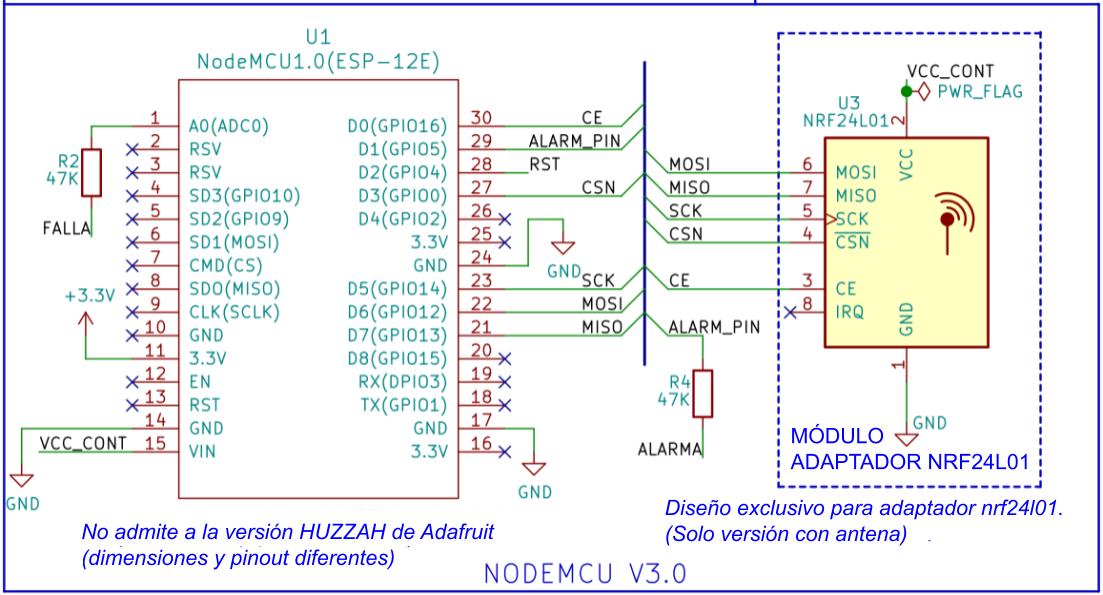
\includegraphics[scale=.3]{./Figures/Capitulo3/Fig_J3.png}
	\caption{Módulo de comunicación inalámbrica de largo alcance.}
	\label{fig:figura_j3}
\end{figure} 


\subsubsection{Módulo de notificación visual}

Debido a restricciones del dispositivo con respecto al número de GPIO disponible el sistema no implementa una conexión directa con el led de notificación de estado normal. En la figura \ref{fig:figura_k3} se puede verificar que el encendido del led indicador del estado normal se realiza a través de hardware ante la ausencia de señales de falla o alarma.

\begin{figure}[]
	\centering
	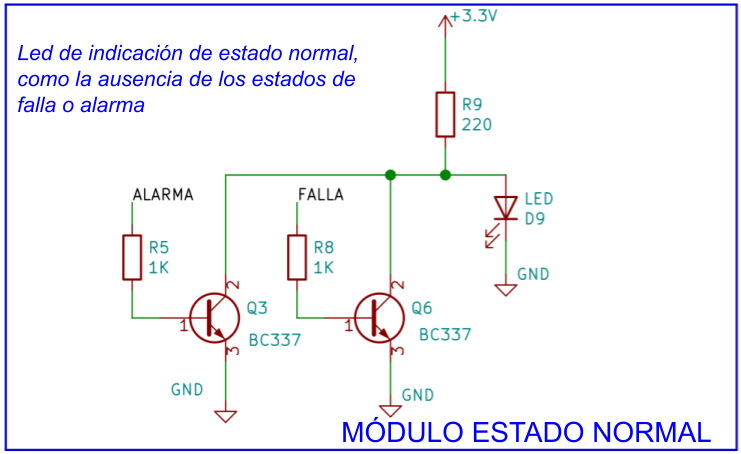
\includegraphics[scale=.35]{./Figures/Capitulo3/Fig_K3.png}
	\caption{Módulo de notificación visual.}
	\label{fig:figura_k3}
\end{figure} 


\subsubsection{Módulo de alimentación}

La alimentación del dispositivo se obtiene a partir del módulo LM2596S-123-3000, un regulador de tensión continua regulable, configurado a 12 vdc. La figura \ref{fig:figura_l3} exhibe al módulo de alimentación y el diseño de una etapa de protección ante casos de conexión con polaridad inversa.

\begin{figure}[]
	\centering
	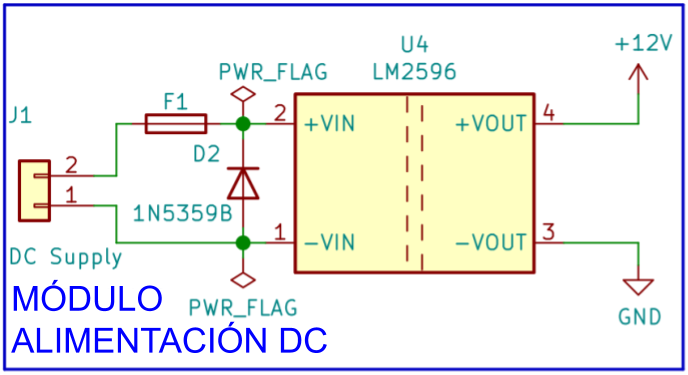
\includegraphics[scale=.3]{./Figures/Capitulo3/Fig_L3.png}
	\caption{Módulo de notificación visual.}
	\label{fig:figura_l3}
\end{figure} 


\section{Software}

Esta sección describe  el funcionamiento de los módulos lógicos más importantes de cada dispositivo; se resaltan las consideraciones y flujo de acciones que rigen en cada caso.

\subsection{Dispositivo primario}

El dispositivo primario funciona a partir del diagrama de flujo de la figura \ref{fig:figura_disp_prim}, para ello utiliza los recursos del sistema operativo Raspbian para la generación de un programa multi hilos, lo que permite desarrollar un sistema escalable y segmentado organizado de la siguiente forma: 

\begin{figure}[]
	\centering
	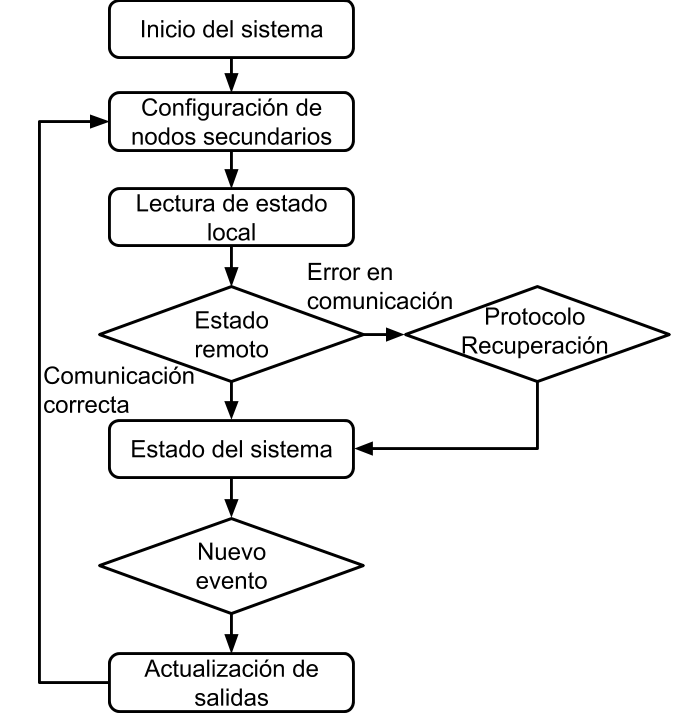
\includegraphics[scale=.3]{./Figures/Capitulo3/Fig_Fl_Pri.png}
	\caption{Diagrama de flujo del dispositivo primario.}
	\label{fig:figura_disp_prim}
\end{figure} 

\begin{itemize}
\item Tareas de actualización: aquellas funcionalidades con mayor prioridad y de ejecución frecuente generan la información que utilizarán las tareas de control para determinar las acciones correspondientes.
\item Tareas de control: este segmento agrupa aquellas funciones dependientes del estado actual y la información obtenida de las tareas de actualización, modifican el estado actual y las salidas del sistema. 
\item Tareas de notificación periódica: el sistema genera una validación cada segundo en la que verifica el estado actual tanto del sistema de detección de incendio, como el del subsistema de comunicación inalámbrica para luego proceder a actualizar los archivos de registro bases de datos del sistema para la actualización de las interfaces de notificación al usuario.
\item Tareas de mantenimiento: las tareas de control tienen la potestad de activar tareas específicas para intentar reponer fallas en el sistema asociadas a la comunicación inalámbrica. Estas funcionalidades otorgan al programa un protocolo de recuperación que permite reiniciar la interfaz de comunicación con el módulo transceptor nrf24l01.
\end{itemize}

La organización del sistema en segmentos de tareas donde cada una se ejecuta con un objetivo específico proporciona una estructura al software que estandariza el proceso de inclusión de nuevas funcionalidades.  A continuación se describe el flujo de los segmentos de código ejecutados por el dispositivo primario:

\subsubsection{Módulo de estado}

El sistema tiene cuatro posibles transiciones:
\begin{itemize}
\item Alarma y falla.
\item Alarma.
\item Falla.
\item Normal.  
\end{itemize}

Este módulo se encarga de definir cuál de estas transiciones debe ser ejecutada. Su funcionamiento requiere evaluar tanto el estado del dispositivo local monitoreado como el cada uno de los estados remotos provenientes de los dispositivos secundarios.

El enfoque utilizado se puede analizar en el diagrama de flujo de la figura \ref{fig:figura_n3}. El sistema funciona a partir de ventanas de tiempo de 200 ms, durante los cuales se registran los siguientes datos de cada mensaje recibido: código de identificación del remitente, código asociado al estado del sistema monitoreado y estado del dispositivo. Los primeros dos elementos provienen del dispositivo secundario que estableció la comunicación, sin embargo el tercer elemento es impuesto por el dispositivo primario, cada vez que el sistema recibe un código establece el estado del nodo como activo. De esta forma se indica qué dispositivos se encuentran comunicándose correctamente.

\begin{figure}[]
	\centering
	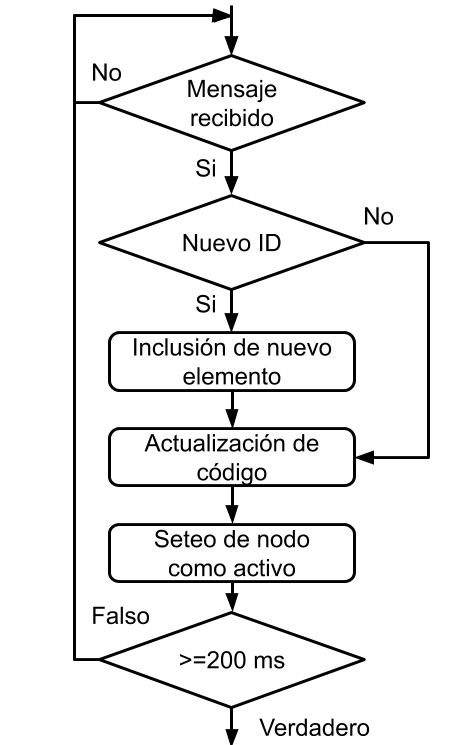
\includegraphics[scale=.35]{./Figures/Capitulo3/Fig_N3.png}
	\caption{Diagrama de flujo del módulo de estado.}
	\label{fig:figura_n3}
\end{figure}  


\subsubsection{Protocolo de recuperación}

Con la intención de generar un sistema que requiera del menor mantenimiento correctivo posible se implementa un protocolo ante fallas de comunicación inalámbrica. El sistema funciona según lo descrito en la figura \ref{fig:figura_o3}. Este busca busca tomar ventaja de las características del módulo nrf24l01 para establecer un sistema de comunicación robusto con la capacidad de recuperarse de forma automática.

\begin{figure}[]
	\centering
	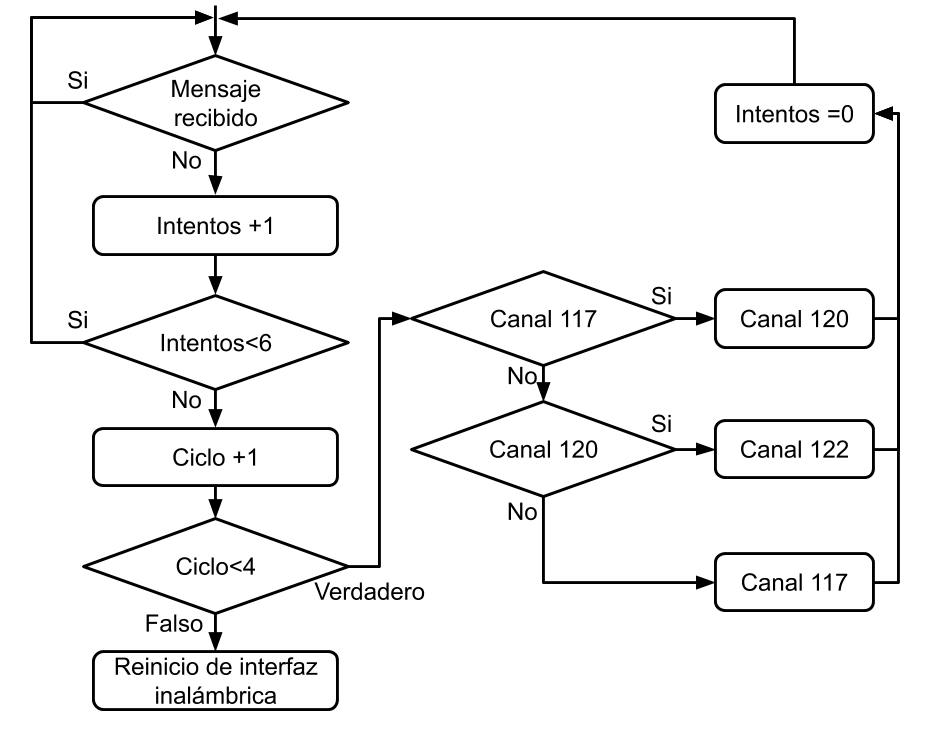
\includegraphics[scale=.35]{./Figures/Capitulo3/Fig_O3.png}
	\caption{Diagrama de flujo del protocolo de recuperación.}
	\label{fig:figura_o3}
\end{figure}  

Este módulo clasifica el estado de la comunicación en cuatro posibles estados: ``sin problemas'',  ``incompleto'',  ``saltando'' y  ``en reparación'', cada uno hace referencia a una etapa del protocolo de recuperación:  

\begin{itemize}
\item Sin problemas: el sistema hace una serie de intentos a una determinada frecuencia; si logra establecer la comunicación con la cantidad de dispositivos secundarios especificada no se presentan fallas de comunicación y se concluye que el sistema funciona correctamente.
\item Saltando: en caso de que el sistema no reciba información de ninguno de los dispositivos secundarios procede a realizar una serie de intentos en la misma frecuencia, hasta alcanzar un número de cinco intentos. Si la falla se mantiene procede a realizar un salto de frecuencia, y reiniciar el conteo de intentos a cero. Este salto se puede realizar un máximo de dos veces por lo que al alcanzar el tercer salto se procederá a la siguiente etapa. 
\item Reparación: el ciclo descrito para el estado ``saltando'' ahora se contabiliza. Si este ciclo de intentos se realiza tres veces consecutivas y no se logra establecer comunicación con ninguno de los dispositivos el sistema procederá a realizar un reinicio de la interfaz con el nodo transceptor nrf24l01+, se eliminan los registros asociados y comienza el ciclo nuevamente.
\item Incompleto: el protocolo de recuperación existe únicamente para casos en los que no se pueda establecer la comunicación con ninguno de los dispositivos secundarios. Si por el contrario al menos un dispositivo secundario se comunica correctamente el protocolo no es ejecutado ya que en esa frecuencia existe un dispositivo. Dependerá del resto de dispositivos secundarios modificar su canal de transmisión para sincronizarse con el dispositivo primario.  
\end{itemize}

\subsubsection{Lógica del sistema}

El dispositivo primario contiene la lógica de las transiciones posibles para el sistema, que se puede analizar a partir del esquema de la figura \ref{fig:figura_p3} que ilustra cómo deben ser los cambios de estado a partir de las condiciones de transición presentes. La figura introduce los  ``estados previos'' que permiten generar acciones antes de la activación de un estado específico y más importante aún, funcionan como un elemento de validación, ya que hacen necesario que la transición entre estados principales (alarma y falla, alarma, normal y falla) se realice únicamente ante dos transiciones del mismo tipo.

\begin{figure}[]
	\centering
	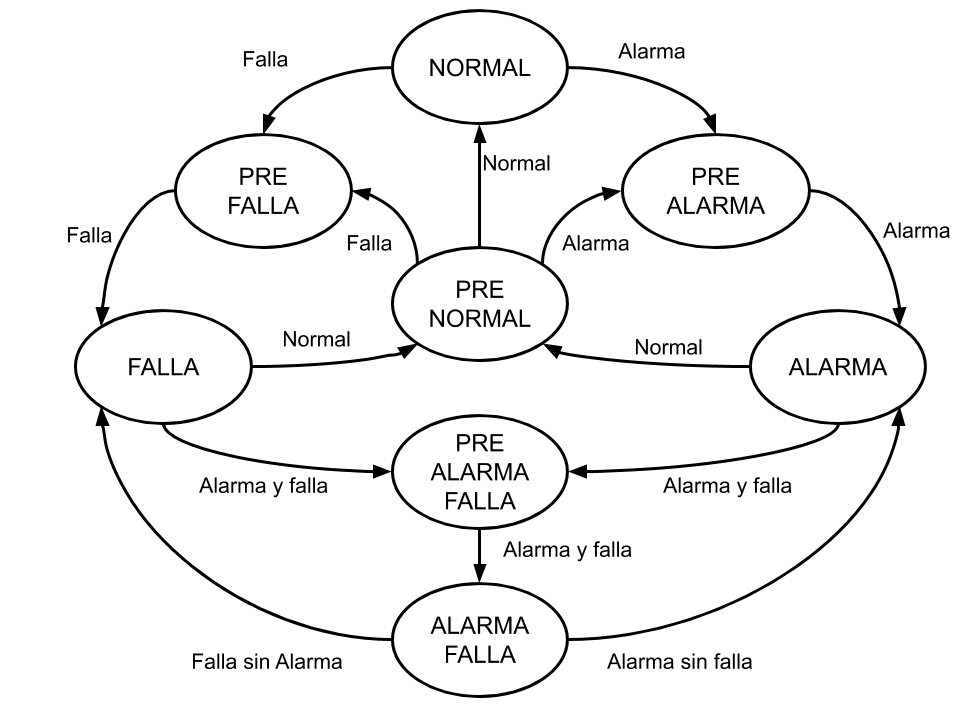
\includegraphics[scale=.35]{./Figures/Capitulo3/Fig_P3.png}
	\caption{Diagrama de flujo de la lógica del sistema.}
	\label{fig:figura_p3}
\end{figure}  

El segmento de código \ref{cod:vControl} se alimenta a partir de la información generada por el módulo de estado. Realiza un análisis con el objetivo de determinar la transición adecuada y la cantidad de dispositivos secundarios activos. Esta información es procesada junto con el estado actual para establecer el nuevo estado y las acciones correspondientes a ejecutar.

\begin{lstlisting}[label=cod:vControl,caption=Pseudocódigo de  de mensajes inalámbricos.]  % Start your code-block

int Comm_Code(RF_List_t* RF_List,Nodes_Database_t* Data_RF_List)
{
	int Final_Code;
	bool Alarm=0;
	bool Fail=0;
	int i;
	int counter=0;
	RF_Device_t * Mem_Block;
		
	Data_RF_List->Counter=0;
	
	
//	- Ciclo de verificacion de estados  

	for(i=0;i<RF_List->counter;i++)
	{	
		Mem_Block=RF_List->RF_Devices[i];
		Update_Node_Data(Mem_Block[0],Data_RF_List,i);

		if(Mem_Block[0].updated)	// El nodo fue actualizado?
		{
			counter++;
			Mem_Block[0].updated=0;
			
			if(ALARM_FAIL_CODE==Mem_Block[0].RF_Code)
			{
				Alarm=1;
				Fail=1;
			}
		
			if(ALARM_CODE==Mem_Block[0].RF_Code)
			{
				Alarm=1;
			}
			
			if(FAIL_CODE==Mem_Block[0].RF_Code)
			{
				Fail=1;
			}
		}
	}
	RF_List->active_nodes = counter; //Registro de cantidad de nodos activos

	if((Alarm)&&(Fail))
	{
		Final_Code = ALARM_FAIL_CODE;
	}else if(Alarm)
	{
		Final_Code = ALARM_CODE;
	}else if(Fail)
	{
		Final_Code = FAIL_CODE;
	}else
	{
		Final_Code = NORMAL_CODE;
	}
	//Si existe al menos una alarma o una falla	el sistema cambia a dicho estado.
	return Final_Code;
}
\end{lstlisting}

% CODIGO!!!!!!!!!!

\subsection{Servicios de interacción con el usuario}

\subsubsection{Interfaz Web}

El software utilizado funciona a partir del monitoreo de cambios recientes en un archivo de registro de eventos, que hace la función de histórico de eventos del sistema. Se valida cada cinco segundos el estado del sistema, y en caso de encontrar diferencias entre el estado anterior y el estado actual, el registro se modifica, lo que provoca una actualización en la plataforma web gestionada por Node-RED.  

La plataforma Node-RED gestiona la interacción con el usuario a nivel local, lo que significa que siempre que el usuario se encuentre conectado a la misma red del sistema de monitoreo de detección de incendio se le otorgará acceso a esta interfaz, que le permitirá configurar del sistema y observar el estado en general. Esta decisión evita la modificación del sistema de detección de incendio de forma remota.         

\subsubsection{Firebase}

La base de datos de Firebase se actualiza a partir del archivo histórico de eventos, de donde se extrae la información más reciente y se carga a partir de un script de Python en el servidor web de Firebase.

Este módulo propone una alternativa para el monitoreo del sistema de forma remota desde cualquier punto con conexión a  Internet. La plataforma brinda un servicio de \textit{realtime database}, que posee integraciones con diferentes elementos como páginas web, aplicaciones Android o IOS. El módulo Firebase no provee al usuario la posibilidad de configurar ningún parámetro. En otras palabras funciona únicamente para monitorear el estado del sistema de forma remota.

\subsubsection{Bases de datos}

Una alternativa al archivo de histórico de eventos es el registro de eventos a través del uso de bases de datos con la biblioteca SQLite; el sistema genera las siguientes bases de datos:
\begin{itemize}
\item Histórico de eventos: registro de cualquier tipo de eventos como alarmas, fallas y cambios en el estado de la comunicación inalámbrica.
\item Detalle de comunicación inalámbrica: se recibe información de diferentes nodos, estos datos quedan registrados y son actualizados cada vez que se establece un nuevo estado remoto. Esto hace posible obtener un detalle de cuáles dispositivos se encuentran comunicándose correctamente con el dispositivo primario.    
\end{itemize}

\subsection{Dispositivo secundario}

Es un dispositivo enfocado en la transmisión del estado del dispositivo monitoreado. La figura \ref{fig:figura_disp_fl_sec} expone el diagrama de flujo utilizado por el sistema. Una vez adquirido el estado del sistema a monitorear se procede a transmitirlo al dispositivo primario y en caso de falla se ejecuta el protocolo de recuperación según corresponda.

El software del dispositivo secundario se basa en un sistema operativo cooperativo que distribuye las funcionalidades del sistema en un arreglo de tareas cada una con un enfoque particular, muy similar a la arquitectura utilizada para el dispositivo primario.

\begin{figure}[]
	\centering
	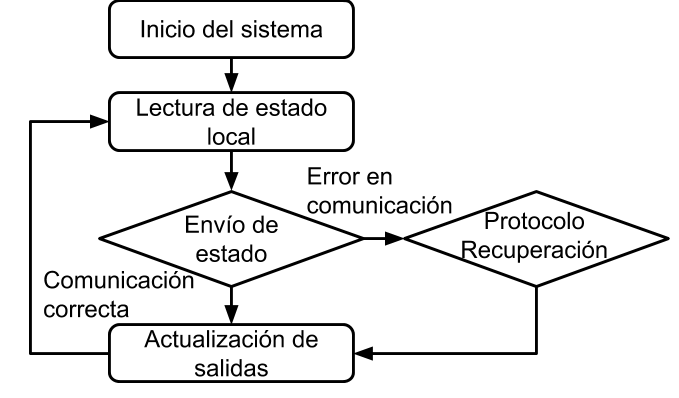
\includegraphics[scale=.35]{./Figures/Capitulo3/Fig_Fl_Sec.png}
	\caption{Diagrama de flujo general del dispositivo secundario.}
	\label{fig:figura_disp_fl_sec}
\end{figure} 
%***********************************************

El dispositivo secundario se resume a una versión del dispositivo primario orientado únicamente a la transmisión del estado actual mediante el módulo nrf24l01.

% Chapter Template

\chapter{Ensayos y Resultados} % Main chapter title

\label{Chapter4} % Change X to a consecutive number; for referencing this chapter elsewhere, use \ref{ChapterX}

%----------------------------------------------------------------------------------------
%	SECTION 1
%----------------------------------------------------------------------------------------

En este capítulo se detallan las pruebas que fueron realizadas sobre los distintos
módulos de hardware y software que componen al robot así como los resultados
de las pruebas de campo que se llevaron a cabo.

Este capítulo contiene la  descripción de las pruebas realizadas para la validación del sistema. Los diferentes ensayos se realizaron sobre los módulos de hardware y software de los dispositivos primario y secundario, inserción  de fallas y pruebas generales del sistema.

\section{Validación de componentes}
\label{sec:validacion_componentes}

Como se explicó anteriormente, los criterios escogidos para la selección de los dispositivos fueron: a) el factor económico, b) nivel de documentación, c) disponibilidad en el mercado argentino, d) tiempo estimado de desarrollo. Sin embargo, el criterio determinante se basó en los resultados generados en los ensayos que se describen a continuación.

\subsection{Uso del Nrf24l01+}

El objetivo de este ensayo fue verificar el uso de la biblioteca RF24 para la transmisión de paquetes de información de forma inalámbrica a través del transceptor nrf24l01+ bajo condiciones ideales.

La prueba consistió  en establecer la comunicación inalámbrica entre dos nodos separados a una distancia de 40 cm. Uno de los nodos mantiene un conteo incremental e intenta transmitir la última lectura al próximo nodo --que se mantiene a la espera del mensaje--. En caso de que transcurra un tiempo mayor o igual a 200 ms sin recibir un mensaje, se registra un evento de timeout. El resultado se obtiene a partir del porcentaje de mensajes erróneos en relación con los totales enviados, durante un periodo de una hora.

%\textit{testing}.
Materiales utilizados:
\begin{itemize}
\item  Nrf24l01 amplificador de potencia con reducción de ruido y antena.
\item  Nrf24l01 + antena PCB.
\item  Arduino Uno.   
\item  NodeMCU v3.
\item  Adafruit Feather HUZZAH ESP8266.
\item  Raspberry Pi.
\item  Fuente de poder Canakit micro USB 2,5 A con filtro de ruido.
\item Adaptador 120-240 VA a 5V DC USB.
\end{itemize}

La figura \ref{fig:figura_a} muestra un esquema de la metodología empleada para realizar la primera prueba de este ensayo. La Raspberry Pi se seleccionó como el único nodo fijo durante estos ensayos. El resto de los dispositivos adoptará sucesivamente el rol de nodo secundario uno a la vez. Los resultados de esta no cubrieron las expectativas esperadas, ya que para cada dispositivo el porcentaje de mensajes exitosos apenas alcanzó un 0,5 \% como máximo.

\vspace{5mm} %5mm vertical space

\begin{figure}[ht]
	\centering
	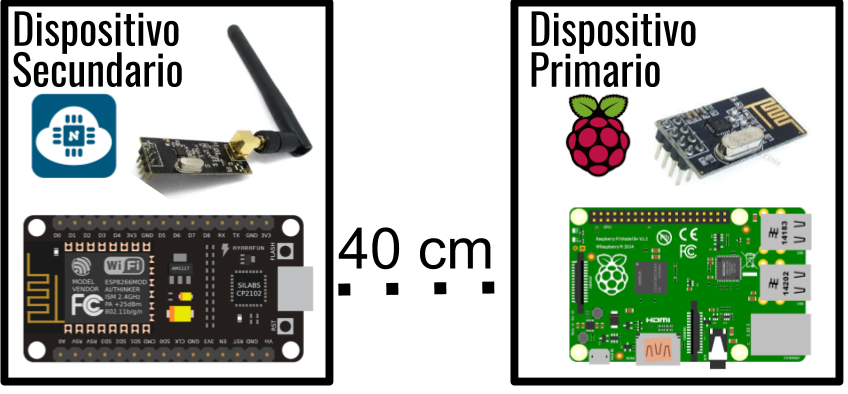
\includegraphics[scale=.45]{./Figures/Capitulo4/Figura_A.png}
	\caption{Esquema utilizado para el ensayo del Nrf24l01+.}
	\label{fig:figura_a}
\end{figure}

Se inició una fase de búsqueda de posibles causas, que comenzó por una revisión de ejemplos de uso del dispositivo --según la documentación de la biblioteca-- así como la revisión de pruebas con resultados similares de diferentes desarrolladores y su experiencia reportada. En función de esto, se identificó que un elemento clave es proveer al dispositivo de una fuente de alimentación estable.

Una vez identificada una posible solución, se reemplazó el adaptador por un equipo de iguales características y de mayor calidad; sen realizó nuevamente el ensayo. Los resultados de esta segunda prueba se consideran satisfactorios y están representados en la figura \ref{fig:figura_b}, en la que se puede apreciar que el menor valor corresponde a un 98 \% de éxito en mensajes transmitidos.


\begin{figure}[ht]
	\centering
	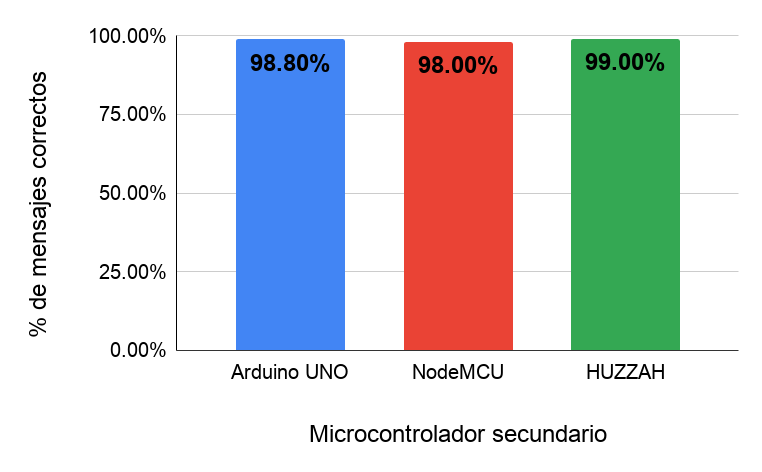
\includegraphics[scale=.45]{./Figures/Capitulo4/Figura_B.png}
	\caption{Resultados del ensayo del Nrf24l01+.}
	\label{fig:figura_b}
\end{figure}

Estos resultados evidencian lo susceptible que es el sistema a ruido en la alimentación y la necesidad de una fuente regulada, estable, con el menor ruido posible. Es por esto que a partir de este punto se incluye en el diseño del sistema el adaptador del módulo transceptor nrf24l01+. Una característica a resaltar de este adaptador es que imposibilita el uso del nrf24l01+ convencional de antena en circuito impreso y es compatible únicamente con el modelo con amplificador de potencia y reducción de ruido con antena.


\subsection{Pruebas de alcance}
 

El objetivo de este ensayo fue verificar el alcance máximo del transceptor nrf24l01+, en diferentes condiciones. La disposición de los equipos utilizados para este ensayo consiste en:

\begin{itemize}
\item Raspberry Pi junto con un transceptor nrf24l01 + de antena interna como dispositivo primario de ubicación fija.
\item Un dispositivo secundario móvil, compuesto por el Arduino UNO y nrf24l01+ de antena interna.
\end{itemize}

Las condiciones en común a las que se exponen los dispositivos son: 
\begin{itemize}
\item Presencia de redes WiFi de diferente intensidad.
\item Equipos electrónicos de bajo consumo.
\end{itemize}

Se procedió a evaluar la respuesta ante situaciones con los siguientes tipos de obstrucción:  
\begin{itemize}
\item Obstrucción nula.
\item Obstrucción total.
	\begin{itemize}
	\item  Puerta de vidrio
	\item  Puerta metálica.
	\end{itemize} 
\end{itemize}  

El propósito de la prueba fue medir la máxima distancia que puede existir entre los nodos primario y secundario, que permita una comunicación inalámbrica estable con una tasa de éxito de al menos 90 \% de mensajes transmitidos. En la figura \ref{fig:figura_c} se puede apreciar la metodología utilizada para el ensayo: se parte de una ubicación inicial, se confirma que la comunicación entre los dispositivos es correcta y se procede a trasladar el dispositivo secundario a una nueva ubicación y repetir nuevamente el proceso de verificación. Se realizó este proceso hasta alcanzar la máxima distancia a la que era posible establecer la comunicación entre los dispositivos. 

\begin{figure}[ht]
	\centering
	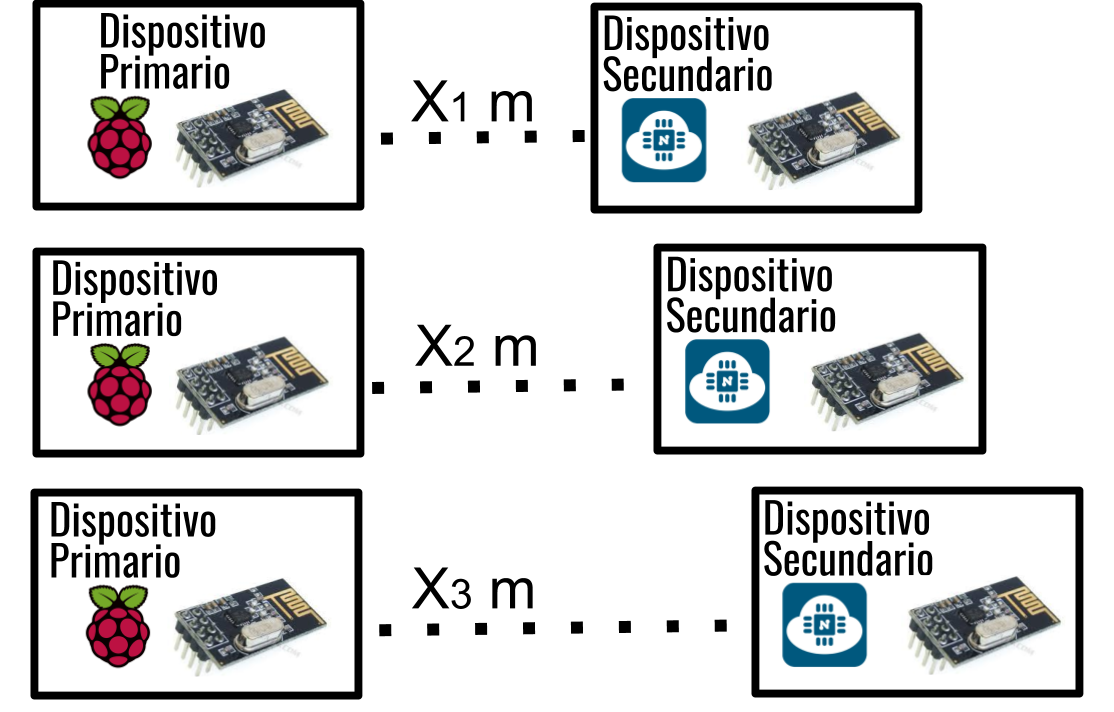
\includegraphics[scale=.3]{./Figures/Capitulo4/Figura_C.png}
	\caption{Esquema del ensayo de la biblioteca RF24.}
	\label{fig:figura_c}
\end{figure}

Los resultados se muestran en la tabla \ref{tab:tabla_1}, donde se puede apreciar la susceptibilidad del sistema ante la obstrucción de objetos sólidos.

\begin{table}[h]
\centering
\caption[Resultados ensayo biblioteca RF24]{Resultados de alcance logrado para el ensayo de la biblioteca RF24}
\begin{tabular}{lccc}
\toprule
\textbf{}                       & \multirow{2}{*}{\textbf{Sin obstáculos}} & \multicolumn{2}{c}{\textbf{Obstrucción total}} \\
\textbf{}                       &                                          & \textbf{Ventanal}  & \textbf{Puerta metálica}  \\
\midrule
\multicolumn{1}{c}{Alcance (m)} & 8,5                                      & 8                  & 0                        
\\
\bottomrule
\hline                                                                        
\end{tabular}
\label{tab:tabla_1}
\end{table}


\subsection{Características de la biblioteca RF24Mesh}

El ensayo anterior establece los valores aproximados de alcance en diferentes condiciones. Para este ensayo se requirió validar el funcionamiento de la biblioteca RF24Mesh con un esquema similar.

Las condiciones de esta prueba consisten en situar dos nodos en ubicaciones fijas separados una distancia de 7 m; con un segundo dispositivo secundario móvil que se utilizará para medir el alcance.

Los resultados del ensayo se pueden observar en la figura \ref{fig:figura_d}: se obtuvo una distancia máxima de 33 m. Al comparar con los resultados del ensayo nrf24l01, se aprecia un incremento en el alcance del sistema, producto de las características del dispositivo secundario 2, ya que este cuenta con un sistema de amplificación de potencia.

\begin{figure}[ht]
	\centering
	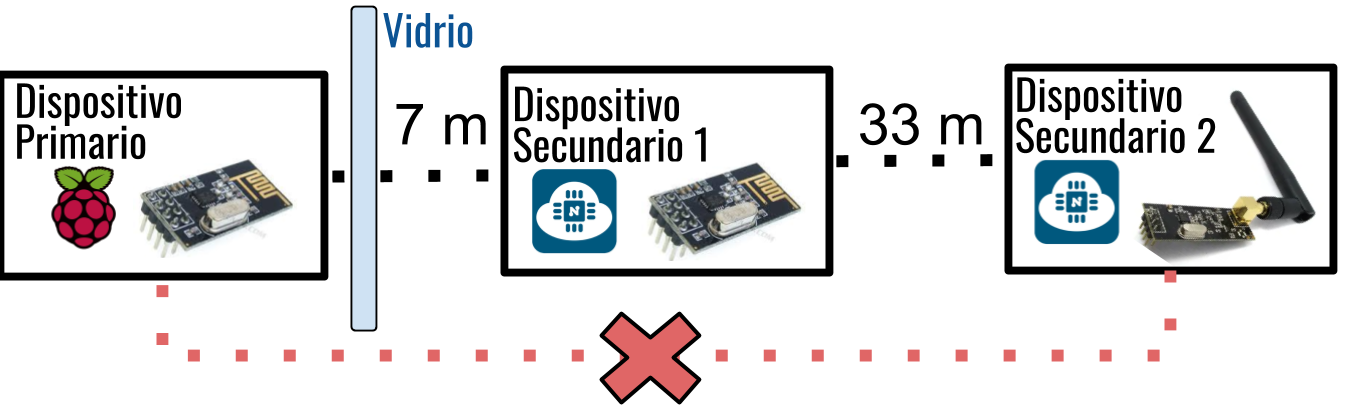
\includegraphics[scale=.3]{./Figures/Capitulo4/Figura_D.png}
	\caption{Resultados del ensayo de la biblioteca RF24Mesh.}
	\label{fig:figura_d}
\end{figure}
\break
Además de la medición del alcance en la nueva configuración de dispositivos inalámbricos, se validan las siguientes funcionalidades de la biblioteca RF24Mesh:


\begin{itemize}
\item Gestión automática de dispositivos conectados: el sistema fue capaz de incluir de manera automática al dispositivo secundario 2 sin necesidad de configuraciones adicionales.
\item Retransmisión de mensajes: el sistema cuenta con la posibilidad de retransmitir los mensajes entre los nodos hasta alcanzar el nodo destino. Esto se comprueba ya que no fue posible establecer la comunicación de forma directa entre el dispositivo secundario 2 y el dispositivo primario. Sin embargo, al existir el dispositivo secundario 1 en la red, este se encarga de recibir el mensaje del dispositivo secundario 2 y transmitirlo al dispositivo primario.
\end{itemize}


\section{Hardware}

Según los requerimientos del sistema, se realizó la fabricación de placas prototipo para la verificación de los diseños de los módulos que componen el sistema. A continuación se presentan los resultados obtenidos del diseño y fabricación de hardware.  

\subsection{Prototipo: dispositivo secundario.}

Inicialmente el objetivo de la fabricación del prototipo era permitir realizar pruebas reales del software durante toda la etapa de desarrollo del trabajo, pero adicional a los aportes de \textit{testing} de software, la elaboración proporcionó la información necesaria para detectar puntos de falla desapercibidos hasta el momento y una reducción importante de costos de producción tanto económicos como de tiempo invertido. En la figura \ref{fig:figura_f} se expone el prototipo realizado.  


\begin{figure}[ht]
	\centering
	\includegraphics[scale=.09]{./Figures/Capitulo4/Figura_F.jpg}
	\caption{Prototipo del dispositivo secundario}
	\label{fig:figura_f}
\end{figure}


A simple vista se puede observar en la figura \ref{fig:figura_e} que el NodeMCU cuenta con GPIOS suficientes para la implementación del dispositivo secundario, ya que el número de recursos disponibles supera el número de recursos requeridos. El diseño descrito en el capítulo \ref{Chapter3} ejecuta un protocolo de reset automático, como parte de un mecanismo de  recuperación ante fallas en la comunicación inalámbrica. Eléctricamente el disparador de este mecanismo es un estado digital alto en el pin RST, lo que implica que es de vital importancia que el pin RST se mantenga en estado digital bajo en todo momento, hasta ser requerido por el algoritmo.

\begin{figure}[ht]
	\centering
	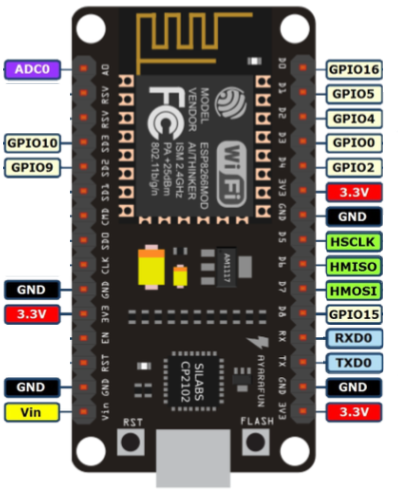
\includegraphics[scale=.55]{./Figures/Capitulo4/Figura_E.png}
	\caption{Resumen de GPIOS de interés para la implementación el sistema.}
	\label{fig:figura_e}
\end{figure}

Durante el encendido del NodeMCU, se ejecuta una secuencia de arranque que altera el estado de diferentes GPIOS. La tabla \ref{tab:tabla_2} muestra un listado de los pines afectados durante el arranque del chip. Al cruzar la información de la figura \ref{fig:figura_e}, con los pines que cumplen la condición de estabilidad durante el arranque según la tabla \ref{tab:tabla_2} podemos inferir que la aseveración realizada anteriormente no es correcta, el número de recursos solicitados es mayor al número de recursos disponibles, lo que hace imposible la implementación del diseño con uso exclusivo de entradas y salidas digitales.

%tabla_2
\begin{table}[h]
\centering
\caption[GPIOS NodeMCU]{Descripción de pines durante arranque de NodeMCU}
\begin{tabular}{ccccc}
\toprule
\textbf{Etiqueta} & \textbf{GPIO} & \textbf{Input}                                               & \textbf{Output} & \textbf{Secuencia de arranque}                                                                 \\
\midrule
D0                & 16            & Sin problema                                                 & Sin problema    & Alto al arranque                                                                               \\
D1                & 5             & Sin problema                                                 & Sin problema    & -                                                                                              \\
D2                & 4             & Sin problema                                                 & Sin problema    & -                                                                                              \\
D3                & 0             & \begin{tabular}[c]{@{}c@{}}Conexión\\ pull up\end{tabular}   & Sin problema    & \begin{tabular}[c]{@{}c@{}}El arranque falla \\ si se encuentra en\\  estado bajo\end{tabular} \\
D4                & 2             & \begin{tabular}[c]{@{}c@{}}Conexión\\ pull up\end{tabular}   & OK              & Alto al arranque                                                                               \\
D5                & 14            & SPI                                                          & SPI             & -                                                                                              \\
D6                & 12            & SPI                                                          & SPI             & -                                                                                              \\
D7                & 13            & SPI                                                          & SPI             & -                                                                                              \\
D8                & 15            & \begin{tabular}[c]{@{}c@{}}Conexión\\ pull down\end{tabular} & OK              & \begin{tabular}[c]{@{}c@{}}El arranque falla\\ si se encuentra en\\ estado alto\end{tabular}   \\
RX                & 3             & UART                                                         & UART            & Alto al arranque                                                                               \\
TX                & 1             & UART                                                         & UART            & Alto al arranque                                                                               \\
A0                & ADC0          & \begin{tabular}[c]{@{}c@{}}Entrada\\ analogica\end{tabular}  & -               & -                                                                                             
\\
\bottomrule
\hline                                                                        
\end{tabular}
\label{tab:tabla_2}
\end{table}


La solución a este problema se centra en aprovechar otra característica del NodeMCU: la medición del voltaje se realizará a través del convertidor analógico digital incluido en el microcontrolador, lo que permite compensar el déficit de GPIOS y mantener el diseño intacto. En concreto se utilizará para el monitoreo del estado del contacto seco de falla.



\subsection{Dispositivos primario y secundario}

Al recopilar la información obtenida de la fabricación de los prototipos, el siguiente paso consistió en consolidar todas estas consideraciones en el esquemático del sistema, con el fin de dar inicio a la fase de elaboración de dispositivos para la fabricación. Las figuras \ref{fig:figura_h} y \ref{fig:figura_i} presentan los circuitos impresos generados en vista 3D y las figuras \ref{fig:disp_prim} y \ref{fig:disp_sec}, las placas fabricadas.

\begin{figure}[ht]
	\centering
	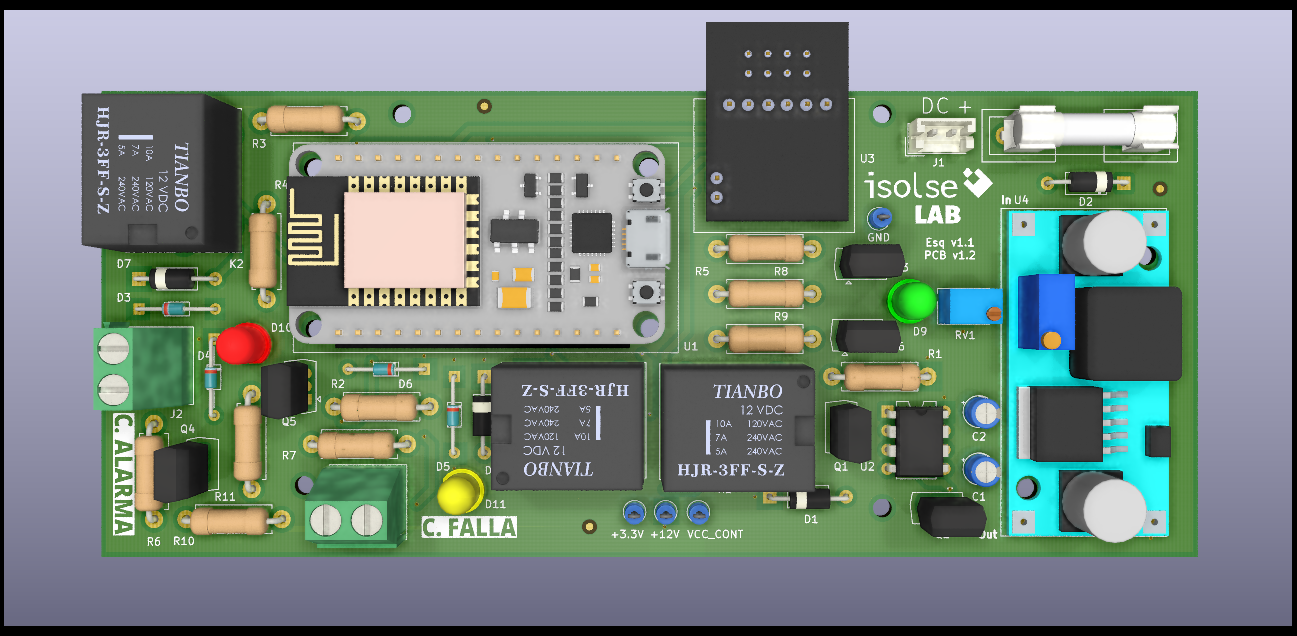
\includegraphics[scale=.25]{./Figures/Capitulo4/Figura_H.png}
	\caption{Vista 3D del diseño de la placa del dispositivo secundario.}
	\label{fig:figura_h}
\end{figure}

\begin{figure}[ht]
	\centering
	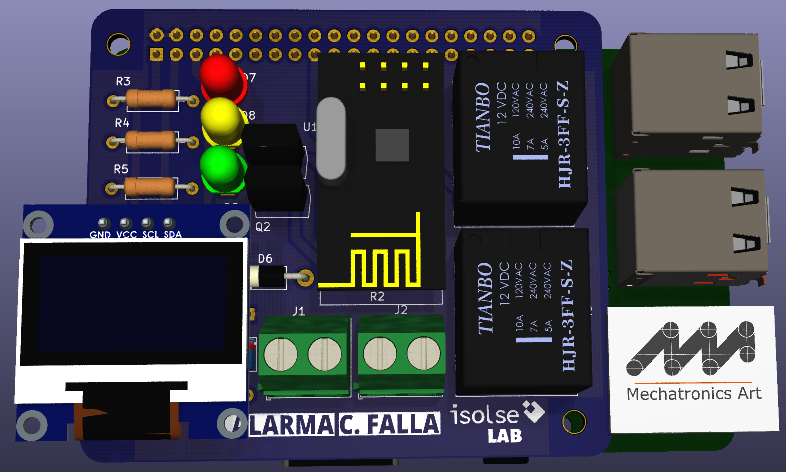
\includegraphics[scale=.3]{./Figures/Capitulo4/Figura_I.png}
	\caption{Vista 3D del diseño de la placa del dispositivo primario.}
	\label{fig:figura_i}
\end{figure}

\begin{figure}[ht]
	\centering
	
\includegraphics[scale=.25]{./Figures/Capitulo4/pendiente.jpg}
	\caption{pediente.}
	\label{fig:disp_prim}
\end{figure}

\begin{figure}[ht]
	\centering
	
\includegraphics[scale=.25]{./Figures/Capitulo4/pendiente.jpg}
	\caption{pediente.}
	\label{fig:disp_sec}
\end{figure}


\section{Pruebas unitarias}

\subsection{Estado local}

Al aplicar la metodología CTM a los casos de pruebas a partir del diseño presentado en el diagrama de la figura \ref{fig:figura_j}. Se obtienen los resultados presentados en la tabla \ref{tab:tabla_3}. Al comparar los resultados obtenidos con los resultados esperados, se concluye que el dispositivo primario funciona correctamente, por lo que a partir de la modificación de los contactos de alarma o falla, se es capaz de establecer correctamente el estado del sistema de monitoreo.


\begin{table}[h]
\centering
\caption[Casos de prueba, estado local]{Casos de prueba del ensayo de sistema con un dispositivo primario.}
\begin{tabular}{clcllc}
\toprule
\textbf{\begin{tabular}[c]{@{}c@{}}Caso de\\ prueba\end{tabular}} & \multicolumn{1}{c}{\textbf{Parámetro}}                                        & \textbf{Valor}           & \multicolumn{2}{c}{\textbf{Comentario}}                                                                                                                                                              & \textbf{\begin{tabular}[c]{@{}c@{}}Resultado\\ esperado\end{tabular}}                                                    \\
\midrule
\multirow{5}{*}{1}                                                & \begin{tabular}[c]{@{}l@{}}Contacto\\ de alarma\end{tabular}                  & Cerrado                  & \multicolumn{2}{l}{\multirow{5}{*}{\begin{tabular}[c]{@{}l@{}}Sistema monitoreado en\\ estado de alarma y falla,\\ al menos una alarma y\\ una falla están presentes\\ en el sistema.\end{tabular}}} & \multirow{5}{*}{\begin{tabular}[c]{@{}c@{}}Led:\\ rojo-amarillo\\ Estado RF:\\ ok\\ Estado:\\ alarma-falla\end{tabular}} \\
                                                                  & \multirow{4}{*}{\begin{tabular}[c]{@{}l@{}}Contacto\\ de falla\end{tabular}}  & \multirow{4}{*}{Cerrado} & \multicolumn{2}{l}{}                                                                                                                                                                                 &                                                                                                                          \\
                                                                  &                                                                               &                          & \multicolumn{2}{l}{}                                                                                                                                                                                 &                                                                                                                          \\
                                                                  &                                                                               &                          & \multicolumn{2}{l}{}                                                                                                                                                                                 &                                                                                                                          \\
                                                                  &                                                                               &                          & \multicolumn{2}{l}{}                                                                                                                                                                                 &                                                                                                                          \\
\multicolumn{1}{l}{}                                              &                                                                               & \multicolumn{1}{l}{}     &                                                                                                   &                                                                                                  & \multicolumn{1}{l}{}                                                                                                     \\
\midrule
\multirow{5}{*}{2}                                                & \begin{tabular}[c]{@{}l@{}}Contacto\\ de alarma\end{tabular}                  & Abierto                  & \multicolumn{2}{l}{\multirow{5}{*}{\begin{tabular}[c]{@{}l@{}}Sistema monitoreado en\\ estado normal, sin fallas\\ ni alarmas presentes.\end{tabular}}}                                              & \multirow{5}{*}{\begin{tabular}[c]{@{}c@{}}Led:\\ verde\\ Estado RF:\\ ok\\ Estado:\\ normal\end{tabular}}               \\
                                                                  & \multirow{4}{*}{\begin{tabular}[c]{@{}l@{}}Contacto\\ de falla\end{tabular}}  & \multirow{4}{*}{Abierto} & \multicolumn{2}{l}{}                                                                                                                                                                                 &                                                                                                                          \\
                                                                  &                                                                               &                          & \multicolumn{2}{l}{}                                                                                                                                                                                 &                                                                                                                          \\
                                                                  &                                                                               &                          & \multicolumn{2}{l}{}                                                                                                                                                                                 &                                                                                                                          \\
                                                                  &                                                                               &                          & \multicolumn{2}{l}{}                                                                                                                                                                                 &                                                                                                                          \\
\multicolumn{1}{l}{}                                              &                                                                               & \multicolumn{1}{l}{}     &                                                                                                   &                                                                                                  & \multicolumn{1}{l}{}                                                                                                     \\
\midrule
\multirow{5}{*}{3}                                                & \begin{tabular}[c]{@{}l@{}}Contacto\\ de alarma\end{tabular}                  & Cerrado                  & \multicolumn{2}{l}{\multirow{5}{*}{\begin{tabular}[c]{@{}l@{}}Sistema monitoreado en\\ estado de alarma, al\\ menos una alarma está\\ presente en el sistema.\end{tabular}}}                         & \multirow{5}{*}{\begin{tabular}[c]{@{}c@{}}Led:\\ rojo\\ Estado RF:\\ ok\\ Estado:\\ alarma\end{tabular}}                \\
                                                                  & \multirow{4}{*}{\begin{tabular}[c]{@{}l@{}}Contacto \\ de falla\end{tabular}} & \multirow{4}{*}{Abierto} & \multicolumn{2}{l}{}                                                                                                                                                                                 &                                                                                                                          \\
                                                                  &                                                                               &                          & \multicolumn{2}{l}{}                                                                                                                                                                                 &                                                                                                                          \\
                                                                  &                                                                               &                          & \multicolumn{2}{l}{}                                                                                                                                                                                 &                                                                                                                          \\
                                                                  &                                                                               &                          & \multicolumn{2}{l}{}                                                                                                                                                                                 &                                                                                                                          \\
\multicolumn{1}{l}{}                                              &                                                                               & \multicolumn{1}{l}{}     &                                                                                                   &                                                                                                  & \multicolumn{1}{l}{}                                                                                                     \\
\midrule
\multirow{5}{*}{4}                                                & \begin{tabular}[c]{@{}l@{}}Contacto\\ de alarma\end{tabular}                  & Abierto                  & \multicolumn{2}{l}{\multirow{5}{*}{\begin{tabular}[c]{@{}l@{}}Sistema monitoreado en\\ estado de falla, al menos\\ una falla está presente\\ en el sistema.\end{tabular}}}                           & \multirow{5}{*}{\begin{tabular}[c]{@{}c@{}}Led:\\ amarillo\\ Estado RF:\\ ok\\ Estado:\\ falla\end{tabular}}             \\
                                                                  & \multirow{4}{*}{\begin{tabular}[c]{@{}l@{}}Contacto\\ de falla\end{tabular}}  & \multirow{4}{*}{Cerrado} & \multicolumn{2}{l}{}                                                                                                                                                                                 &                                                                                                                          \\
                                                                  &                                                                               &                          & \multicolumn{2}{l}{}                                                                                                                                                                                 &                                                                                                                          \\
                                                                  &                                                                               &                          & \multicolumn{2}{l}{}                                                                                                                                                                                 &                                                                                                                          \\
                                                                  &                                                                               &                          & \multicolumn{2}{l}{}                                                                                                                                                                                 &                                                                                                                          \\
\multicolumn{1}{l}{}                                              &                                                                               & \multicolumn{1}{l}{}     &                                                                                                   &                                                                                                  & \multicolumn{1}{l}{}                                                                                                    
\\
\bottomrule
\hline                                                                        
\end{tabular}
\label{tab:tabla_3}
\end{table}

\begin{figure}[ht]
	\centering
	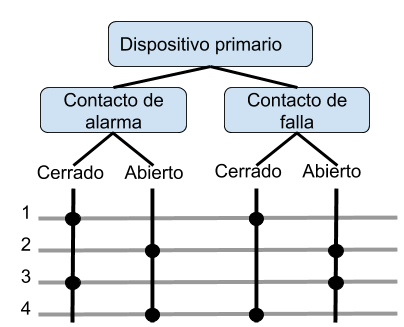
\includegraphics[scale=.5]{./Figures/Capitulo4/Figura_J.png}
	\caption{Diagrama CTM para ensayo de estado local.}
	\label{fig:figura_j}
\end{figure}

\subsection{Sistema con un dispositivo secundario}

Al emplear la misma metodología del ensayo número uno, se generaron la figura \ref{fig:figura_k} y la tabla \ref{tab:tabla_4_1} y \ref{tab:tabla_4_2}, que describen el detalle del ensayo. Se confirma que todos los casos de prueba son ejecutados de forma satisfactoria, por lo que hasta este punto se puede concluir que el dispositivo primario es capaz de comunicarse de forma inalámbrica con un dispositivo secundario, y además puede definir el estado correspondiente del sistema de detección, a partir de su estado propio y el estado del dispositivo secundario. 

\begin{figure}[ht]
	\centering
	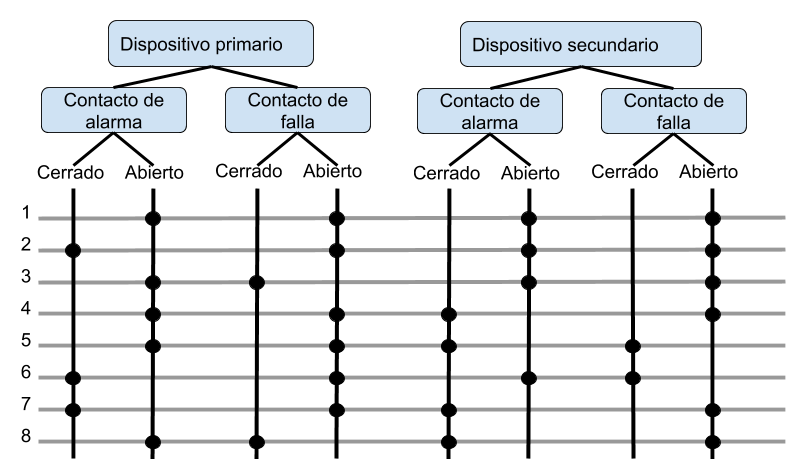
\includegraphics[scale=.45]{./Figures/Capitulo4/Figura_K.png}
	\caption{Diagrama CTM para ensayo con un dispositivo secundario.}
	\label{fig:figura_k}
\end{figure}


\begin{table}[h]
\centering
\caption[Casos de prueba, dispositivo secundario ]{Casos de prueba del ensayo de sistema con un dispositivo secundario.}
\begin{tabular}{clcllc}
\toprule
\textbf{\begin{tabular}[c]{@{}c@{}}Caso de\\ prueba\end{tabular}} & \multicolumn{1}{c}{\textbf{Parámetro}}                                            & \textbf{Valor}           & \multicolumn{2}{c}{\textbf{Comentario}}                                                                                                                                                                                                                                                 & \textbf{\begin{tabular}[c]{@{}c@{}}Resultado\\ esperado\end{tabular}}                                        \\
\midrule
\multirow{5}{*}{1}   
                                             & \begin{tabular}[c]{@{}l@{}}D.P. Contacto\\ de alarma\end{tabular}                 & Abierto                  & \multicolumn{2}{l}{\multirow{5}{*}{\begin{tabular}[c]{@{}l@{}}Ambos sistemas en estado\\ normal, sin fallas ni\\ alarmas presentes.\end{tabular}}}                                                                                                                                       & \multirow{5}{*}{\begin{tabular}[c]{@{}c@{}}Led:\\ verde\\ Estado RF:\\ ok\\ Estado:\\ normal\end{tabular}}   \\
                                                                  & \begin{tabular}[c]{@{}l@{}}D.P. Contacto\\ de falla\end{tabular}                  & Abierto                  & \multicolumn{2}{l}{}                                                                                                                                                                                                                                                                    &                                                                                                              \\
                                                                  & \begin{tabular}[c]{@{}l@{}}D.S. Contacto\\ de alarma\end{tabular}                 & Abierto                  & \multicolumn{2}{l}{}                                                                                                                                                                                                                                                                    &                                                                                                              \\
                                                                  & \multirow{2}{*}{\begin{tabular}[c]{@{}l@{}}D.S. Contacto\\ de falla\end{tabular}} & \multirow{2}{*}{Abierto} & \multicolumn{2}{l}{}                                                                                                                                                                                                                                                                    &                                                                                                              \\
                                                                  &                                                                                   &                          & \multicolumn{2}{l}{}                                                                                                                                                                                                                                                                    &                                                                                                              \\
\multicolumn{1}{l}{}                                              &                                                                                   & \multicolumn{1}{l}{}     &                                                                                                                                            &                                                                                                                                            & \multicolumn{1}{l}{}                                                                                         \\
\midrule
\multirow{7}{*}{2}                                                & \begin{tabular}[c]{@{}l@{}}D.P. Contacto\\ de alarma\end{tabular}                 & Cerrado                  & \multicolumn{2}{l}{\multirow{7}{*}{\begin{tabular}[c]{@{}l@{}}Dispositivo primario: \\ sistema en estado de \\ alarma, al menos una\\ alarma presente en \\ el sistema. \\ \\ Dispositivo secundario:\\ sistema en estado \\ normal, sin fallas ni \\ alarmas presentes.\end{tabular}}} & \multirow{7}{*}{\begin{tabular}[c]{@{}c@{}}Led:\\ rojo\\ Estado RF:\\ ok\\ Estado:\\ alarma\end{tabular}}    \\
                                                                  & \begin{tabular}[c]{@{}l@{}}D.P. Contacto\\ de falla\end{tabular}                  & Abierto                  & \multicolumn{2}{l}{}                                                                                                                                                                                                                                                                    &                                                                                                              \\
                                                                  & \begin{tabular}[c]{@{}l@{}}D.S. Contacto\\ de alarma\end{tabular}                 & Abierto                  & \multicolumn{2}{l}{}                                                                                                                                                                                                                                                                    &                                                                                                              \\
                                                                  & \multirow{4}{*}{\begin{tabular}[c]{@{}l@{}}D.S. Contacto\\ de falla\end{tabular}} & \multirow{4}{*}{Abierto} & \multicolumn{2}{l}{}                                                                                                                                                                                                                                                                    &                                                                                                              \\
                                                                  &                                                                                   &                          & \multicolumn{2}{l}{}                                                                                                                                                                                                                                                                    &                                                                                                              \\
                                                                  &                                                                                   &                          & \multicolumn{2}{l}{}                                                                                                                                                                                                                                                                    &                                                                                                              \\
                                                                  &                                                                                   &                          & \multicolumn{2}{l}{}                                                                                                                                                                                                                                                                    &                                                                                                              \\
\multicolumn{1}{l}{}                                              &                                                                                   & \multicolumn{1}{l}{}     &                                                                                                                                            &                                                                                                                                            & \multicolumn{1}{l}{}                                                                                         \\
\midrule
\multirow{7}{*}{3}                                                & \begin{tabular}[c]{@{}l@{}}D.P. Contacto\\ de alarma\end{tabular}                 & Abierto                  & \multicolumn{2}{l}{\multirow{7}{*}{\begin{tabular}[c]{@{}l@{}}Dispositivo primario:\\ sistema en estado de\\ falla, al menos una\\ falla presente en\\ el sistema. \\ \\ Dispositivo secundario:\\ sistema en estado\\ normal, sin fallas\\ ni alarmas presentes.\end{tabular}}}        & \multirow{7}{*}{\begin{tabular}[c]{@{}c@{}}Led:\\ amarillo\\ Estado RF:\\ ok\\ Estado:\\ falla\end{tabular}} \\
                                                                  & \begin{tabular}[c]{@{}l@{}}D.P. Contacto\\ de falla\end{tabular}                  & Cerrado                  & \multicolumn{2}{l}{}                                                                                                                                                                                                                                                                    &                                                                                                              \\
                                                                  & \begin{tabular}[c]{@{}l@{}}D.S. Contacto\\ de alarma\end{tabular}                 & Abierto                  & \multicolumn{2}{l}{}                                                                                                                                                                                                                                                                    &                                                                                                              \\
                                                                  & \multirow{4}{*}{\begin{tabular}[c]{@{}l@{}}D.S. Contacto\\ de falla\end{tabular}} & \multirow{4}{*}{Abierto} & \multicolumn{2}{l}{}                                                                                                                                                                                                                                                                    &                                                                                                              \\
                                                                  &                                                                                   &                          & \multicolumn{2}{l}{}                                                                                                                                                                                                                                                                    &                                                                                                              \\
                                                                  &                                                                                   &                          & \multicolumn{2}{l}{}                                                                                                                                                                                                                                                                    &                                                                                                              \\
                                                                  &                                                                                   &                          & \multicolumn{2}{l}{}                                                                                                                                                                                                                                                                    &                                                                                                              \\
\multicolumn{1}{l}{}                                              &                                                                                   & \multicolumn{1}{l}{}     &                                                                                                                                            &                                                                                                                                            & \multicolumn{1}{l}{}                                                                                         \\
\midrule
\multirow{7}{*}{4}                                                & \begin{tabular}[c]{@{}l@{}}D.P. Contacto\\ de alarma\end{tabular}                 & Abierto                  & \multicolumn{2}{l}{\multirow{7}{*}{\begin{tabular}[c]{@{}l@{}}Dispositivo primario:\\ sistema en estado \\ normal, sin fallas ni\\ alarmas presentes. \\ \\ Dispositivo secundario:\\ sistema en estado de\\ alarma, al menos una\\ alarma presente en el\\ sistema.\end{tabular}}}      & \multirow{7}{*}{\begin{tabular}[c]{@{}c@{}}Led:\\ rojo\\ Estado RF:\\ ok\\ Estado:\\ alarma\end{tabular}}    \\
                                                                  & \begin{tabular}[c]{@{}l@{}}D.P. Contacto\\ de falla\end{tabular}                  & Abierto                  & \multicolumn{2}{l}{}                                                                                                                                                                                                                                                                    &                                                                                                              \\
                                                                  & \begin{tabular}[c]{@{}l@{}}D.S. Contacto\\ de alarma\end{tabular}                 & Cerrado                  & \multicolumn{2}{l}{}                                                                                                                                                                                                                                                                    &                                                                                                              \\
                                                                  & \multirow{4}{*}{\begin{tabular}[c]{@{}l@{}}D.S. Contacto\\ de falla\end{tabular}} & \multirow{4}{*}{Abierto} & \multicolumn{2}{l}{}                                                                                                                                                                                                                                                                    &                                                                                                              \\
                                                                  &                                                                                   &                          & \multicolumn{2}{l}{}                                                                                                                                                                                                                                                                    &                                                                                                              \\
                                                                  &                                                                                   &                          & \multicolumn{2}{l}{}                                                                                                                                                                                                                                                                    &                                                                                                              \\
                                                                  &                                                                                   &                          & \multicolumn{2}{l}{}                                                                                                                                                                                                                                                                    &                                                                                                              \\
\multicolumn{1}{l}{}                                              &                                                                                   & \multicolumn{1}{l}{}     &                                                                                                                                            &                                                                                                                                            & \multicolumn{1}{l}{}                                                                                        
\\
\bottomrule
\hline                                                                        
\end{tabular}
\label{tab:tabla_4_1}
\end{table}


\begin{table}[h]
\centering
\caption[Continuación de la tabla \ref{tab:tabla_4_1}]{Casos de prueba del ensayo de sistema con un dispositivo secundario.}
\begin{tabular}{clcllc}
\toprule
\textbf{\begin{tabular}[c]{@{}c@{}}Caso de\\ prueba\end{tabular}} & \multicolumn{1}{c}{\textbf{Parámetro}}                                            & \textbf{Valor}           & \multicolumn{2}{c}{\textbf{Comentario}}                                                                                                                                                                                                                                                                         & \textbf{\begin{tabular}[c]{@{}c@{}}Resultado\\ esperado\end{tabular}}                                                    \\
\midrule
\multirow{8}{*}{5}                                                & \begin{tabular}[c]{@{}l@{}}D.P. Contacto\\ de alarma\end{tabular}                 & Abierto                  & \multicolumn{2}{l}{\multirow{8}{*}{\begin{tabular}[c]{@{}l@{}}Dispositivo primario:\\ sistema en estado\\ normal, sin fallas ni\\ alarmas presentes. \\ \\ Dispositivo secundario:\\ sistema en estado de\\ alarma y falla, al menos\\ una alarma y una falla\\ están presentes en el\\ sistema.\end{tabular}}} & \multirow{8}{*}{\begin{tabular}[c]{@{}c@{}}Led:\\ rojo-amarillo\\ Estado RF:\\ ok\\ Estado:\\ alarma-falla\end{tabular}} \\
                                                                  & \begin{tabular}[c]{@{}l@{}}D.P. Contacto\\ de falla\end{tabular}                  & Abierto                  & \multicolumn{2}{l}{}                                                                                                                                                                                                                                                                                            &                                                                                                                          \\
                                                                  & \begin{tabular}[c]{@{}l@{}}D.S. Contacto\\ de alarma\end{tabular}                 & Cerrado                  & \multicolumn{2}{l}{}                                                                                                                                                                                                                                                                                            &                                                                                                                          \\
                                                                  & \multirow{5}{*}{\begin{tabular}[c]{@{}l@{}}D.S. Contacto\\ de falla\end{tabular}} & \multirow{5}{*}{Cerrado} & \multicolumn{2}{l}{}                                                                                                                                                                                                                                                                                            &                                                                                                                          \\
                                                                  &                                                                                   &                          & \multicolumn{2}{l}{}                                                                                                                                                                                                                                                                                            &                                                                                                                          \\
                                                                  &                                                                                   &                          & \multicolumn{2}{l}{}                                                                                                                                                                                                                                                                                            &                                                                                                                          \\
                                                                  &                                                                                   &                          & \multicolumn{2}{l}{}                                                                                                                                                                                                                                                                                            &                                                                                                                          \\
                                                                  &                                                                                   &                          & \multicolumn{2}{l}{}                                                                                                                                                                                                                                                                                            &                                                                                                                          \\
\multicolumn{1}{l}{}                                              &                                                                                   & \multicolumn{1}{l}{}     &                                                                                                                                                        &                                                                                                                                                        & \multicolumn{1}{l}{}                                                                                                     \\
\midrule
\multirow{7}{*}{6}                                                & \begin{tabular}[c]{@{}l@{}}D.P. Contacto\\ de alarma\end{tabular}                 & Cerrado                  & \multicolumn{2}{l}{\multirow{7}{*}{\begin{tabular}[c]{@{}l@{}}Dispositivo primario:\\ sistema en estado\\ de alarma, al menos\\ una alarma presente\\ en el sistema.\\ \\ Dispositivo secundario:\\ sistema en estado de\\ falla, al menos una falla\\ presente en el sistema.\end{tabular}}}                   & \multirow{7}{*}{\begin{tabular}[c]{@{}c@{}}Led:\\ rojo-amarillo\\ Estado RF:\\ ok\\ Estado:\\ alarma-falla\end{tabular}} \\
                                                                  & \begin{tabular}[c]{@{}l@{}}D.P. Contacto\\ de falla\end{tabular}                  & Abierto                  & \multicolumn{2}{l}{}                                                                                                                                                                                                                                                                                            &                                                                                                                          \\
                                                                  & \begin{tabular}[c]{@{}l@{}}D.S. Contacto\\ de alarma\end{tabular}                 & Abierto                  & \multicolumn{2}{l}{}                                                                                                                                                                                                                                                                                            &                                                                                                                          \\
                                                                  & \multirow{4}{*}{\begin{tabular}[c]{@{}l@{}}D.S. Contacto\\ de falla\end{tabular}} & \multirow{4}{*}{Cerrado} & \multicolumn{2}{l}{}                                                                                                                                                                                                                                                                                            &                                                                                                                          \\
                                                                  &                                                                                   &                          & \multicolumn{2}{l}{}                                                                                                                                                                                                                                                                                            &                                                                                                                          \\
                                                                  &                                                                                   &                          & \multicolumn{2}{l}{}                                                                                                                                                                                                                                                                                            &                                                                                                                          \\
                                                                  &                                                                                   &                          & \multicolumn{2}{l}{}                                                                                                                                                                                                                                                                                            &                                                                                                                          \\
\multicolumn{1}{l}{}                                              &                                                                                   & \multicolumn{1}{l}{}     &                                                                                                                                                        &                                                                                                                                                        & \multicolumn{1}{l}{}                                                                                                     \\
\midrule
\multirow{8}{*}{7}                                                & \begin{tabular}[c]{@{}l@{}}D.P. Contacto\\ de alarma\end{tabular}                 & Cerrado                  & \multicolumn{2}{l}{\multirow{8}{*}{\begin{tabular}[c]{@{}l@{}}Dispositivo primario: \\ sistema en estado \\ de alarma, al menos\\ una alarma presente\\ en el sistema.\\ \\ Dispositivo secundario:\\ sistema en estado de\\ alarma, al menos una\\ alarmapresente en el\\ sistema.\end{tabular}}}              & \multirow{8}{*}{\begin{tabular}[c]{@{}c@{}}Led:\\ rojo\\ Estado RF:\\ ok\\ Estado:\\ alarma\end{tabular}}                \\
                                                                  & \begin{tabular}[c]{@{}l@{}}D.P. Contacto\\ de falla\end{tabular}                  & Abierto                  & \multicolumn{2}{l}{}                                                                                                                                                                                                                                                                                            &                                                                                                                          \\
                                                                  & \begin{tabular}[c]{@{}l@{}}D.S. Contacto\\ de alarma\end{tabular}                 & Cerrado                  & \multicolumn{2}{l}{}                                                                                                                                                                                                                                                                                            &                                                                                                                          \\
                                                                  & \multirow{5}{*}{\begin{tabular}[c]{@{}l@{}}D.S. Contacto\\ de falla\end{tabular}} & \multirow{5}{*}{Abierto} & \multicolumn{2}{l}{}                                                                                                                                                                                                                                                                                            &                                                                                                                          \\
                                                                  &                                                                                   &                          & \multicolumn{2}{l}{}                                                                                                                                                                                                                                                                                            &                                                                                                                          \\
                                                                  &                                                                                   &                          & \multicolumn{2}{l}{}                                                                                                                                                                                                                                                                                            &                                                                                                                          \\
                                                                  &                                                                                   &                          & \multicolumn{2}{l}{}                                                                                                                                                                                                                                                                                            &                                                                                                                          \\
                                                                  &                                                                                   &                          & \multicolumn{2}{l}{}                                                                                                                                                                                                                                                                                            &                                                                                                                          \\
\multicolumn{1}{l}{}                                              &                                                                                   & \multicolumn{1}{l}{}     &                                                                                                                                                        &                                                                                                                                                        & \multicolumn{1}{l}{}                                                                                                     \\
\midrule
\multirow{6}{*}{8}                                                & \begin{tabular}[c]{@{}l@{}}D.P. Contacto\\ de alarma\end{tabular}                 & Abierto                  & \multicolumn{2}{l}{\multirow{6}{*}{\begin{tabular}[c]{@{}l@{}}Dispositivo primario:\\ sistema en estado\\ de falla, al menos\\ una falla presente\\ en el sistema.\\ \\ Dispositivo secundario:\\ sistema en estado de\\
alarma.\end{tabular}}}                 & \multirow{6}{*}{\begin{tabular}[c]{@{}c@{}}Led:\\ rojo-amarillo\\ Estado RF:\\ ok\\ Estado:\\ alarma-falla\end{tabular}} \\
                                                                  & \begin{tabular}[c]{@{}l@{}}D.P. Contacto\\ de falla\end{tabular}                  & Cerrado                  & \multicolumn{2}{l}{}                                                                                                                                                                                                                                                                                            &                                                                                                                          \\
                                                                  & \begin{tabular}[c]{@{}l@{}}D.S. Contacto\\ de alarma\end{tabular}                 & Cerrado                  & \multicolumn{2}{l}{}                                                                                                                                                                                                                                                                                            &                                                                                                                          \\
                                                                  & \multirow{3}{*}{\begin{tabular}[c]{@{}l@{}}D.S. Contacto\\ de falla\end{tabular}} & \multirow{3}{*}{Abierto} & \multicolumn{2}{l}{}                                                                                                                                                                                                                                                                                            &                                                                                                                          \\
                                                                  &                                                                                   &                          & \multicolumn{2}{l}{}                                                                                                                                                                                                                                                                                            &                                                                                                                          \\
                                                                  &                                                                                   &                          & \multicolumn{2}{l}{}                                                                                                                                                                                                                                                                                            &                                                                                                                          \\
\multicolumn{1}{l}{}                                              &                                                                                   & \multicolumn{1}{l}{}     &                                                                                                                                                        &                                                                                                                                                        & \multicolumn{1}{l}{}                                                                                                    
\\
\bottomrule
\hline                                                                        
\end{tabular}
\label{tab:tabla_4_2}
\end{table}

\subsection{Sistema con dos dispositivos secundarios.}

Se mantiene la estrategia para el diseño de casos de prueba. Los resultados se muestran en la figura \ref{fig:figura_l}. Para realizar este ensayo se incluyó un nodo que permanecerá en estado de alarma durante todos los casos de prueba. Los resultados que se obtuvieron en esta prueba son insatisfactorios.

\begin{figure}[ht]
	\centering
	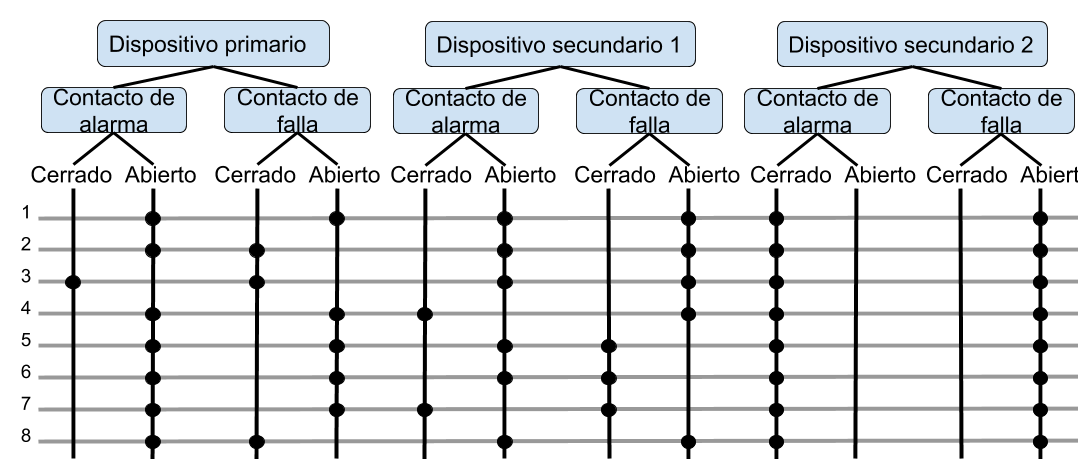
\includegraphics[scale=.35]{./Figures/Capitulo4/Figura_L.png}
	\caption{Diagrama CTM para sistema con dos dispositivos secundarios.}
	\label{fig:figura_l}
\end{figure}

Los casos de prueba fallaron debido a que el sistema fue incapaz de responder de forma correcta en un tiempo menor a 10 s. Al analizar el algoritmo de gestión de comunicación inalámbrica en el dispositivo primario y compararlo con el algoritmo de transmisión de paquetes, se descubrió que el dispositivo secundario estaba configurado para la transmisión de información cada 15 ms y el dispositivo primario disponía de 10 ms como ventana de tiempo para hacer el análisis del sistema. 

Ello generaba un comportamiento inestable, al no poder asegurar que el dispositivo primario reciba la información de todos los nodos que conforman la red en un tiempo tan reducido. Un problema adicional que se presentó fue la acumulación de mensajes, ya que al no leer el mensaje, el sistema lo guarda para su procesamiento en la siguiente llamada, esto generaba retrasos de hasta 15 segundos en la actualización del estado. Al identificar la causa del problema, se planteó una modificación de los tiempos configurados para la comunicación inalámbrica en ambos dispositivos. 

Los nuevos parámetros establecidos para la comunicación son 200 ms para el dispositivo primario y 30 ms para el dispositivo secundario. Esta nueva configuración permitió cumplir correctamente los casos de prueba.

      
Un punto de mejora que resulta de la realización de este ensayo es la posibilidad de incluir una interfaz que permita facilitar la inclusión de dispositivos al sistema, ya que la metodología actual de trabajo hace imposible al usuario incluir un nodo sin conocer el funcionamiento del código y su estructura.

\subsection{Sistema con tres dispositivos secundarios}

Basados en la información recopilada de los ensayos previos, se propuso elaborar un nuevo ensayo con un nodo adicional, esta vez con la intención de validar si la configuración de tiempo utilizada fue adecuada. El ensayo incluyó un nodo con un estado de sistema estático. En este caso el nuevo nodo permanecerá en estado normal durante todos los casos de prueba, con el propósito de validar la velocidad de respuesta del sistema. El ensayo logró confirmar el correcto funcionamiento del sistema con la configuración de parámetros seleccionada en el ensayo con dos dispositivos secundarios.

\subsection{Protocolo de recuperación}

El ensayo se orientó exclusivamente en comprobar el funcionamiento de la lógica de módulo de recuperación ante fallas de comunicación inalámbrica. Se utilizó el esquema de la figura \ref{fig:ctm_protocolo} y se generan los casos de prueba de la tabla \ref{tab:protocolo}.


\begin{figure}[ht]
	\centering
	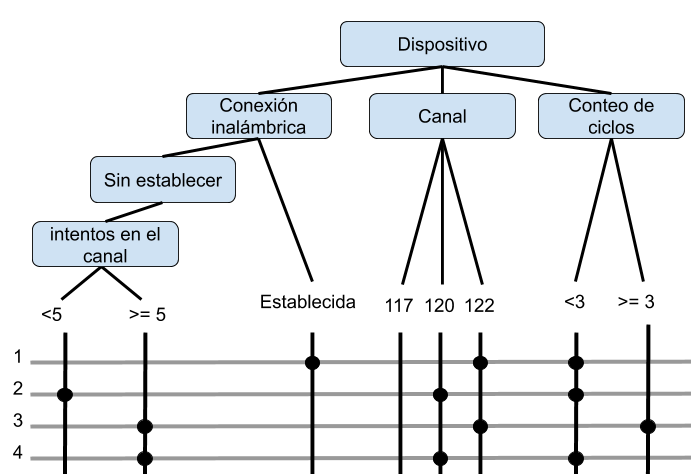
\includegraphics[scale=.4]{./Figures/Capitulo4/CTM_PROTOCOLO.png}
	\caption{Diagrama CTM para protocolo de recuperación ante fallas de comunicación inalámbrica.}
	\label{fig:ctm_protocolo}
\end{figure}


%\begin{table}[h]
%\centering
%\caption[Casos de prueba protocolo ante fallas]{Casos de prueba del ensayo de protocolo de recuperación.}
%\begin{tabular}{cllll}
%\toprule
%\\
%\bottomrule
%\hline                                                                        
%\end{tabular}
%\label{tab:protocolo}
%\end{table}


\begin{table}[h]
\centering
\caption[Casos de prueba protocolo ante fallas]{Casos de prueba del ensayo de protocolo de recuperación.}
\begin{tabular}{cllll}
\toprule
\textbf{\begin{tabular}[c]{@{}c@{}}Caso de\\ prueba\end{tabular}} & \multicolumn{1}{c}{\textbf{Parámetro}}                         & \multicolumn{1}{c}{\textbf{Valor}}                             & \multicolumn{1}{c}{\textbf{Comentario}}                                                                                                                             & \multicolumn{1}{c}{\textbf{\begin{tabular}[c]{@{}c@{}}Resultado\\ esperado\end{tabular}}}                                                          \\
\midrule
\multirow{5}{*}{1}                                                & \begin{tabular}[c]{@{}l@{}}Conexión\\ inalámbrica\end{tabular} & Establecida                                                    & \multirow{5}{*}{\begin{tabular}[c]{@{}l@{}}Comunicación\\ inalámbrica\\ funciona \\ correctamente \\ en el canal 122.\end{tabular}}                                & \multirow{5}{*}{\begin{tabular}[c]{@{}l@{}}Permanecer en\\ el canal 122,\\ reinicio de\\ conteos de\\ intentos.\end{tabular}}                      \\
                                                                  & Canal                                                          & 122                                                            &                                                                                                                                                                     &                                                                                                                                                    \\
                                                                  & \begin{tabular}[c]{@{}l@{}}Conteo de \\ ciclos\end{tabular}    & 1                                                              &                                                                                                                                                                     &                                                                                                                                                    \\
                                                                  &                                                                &                                                                &                                                                                                                                                                     &                                                                                                                                                    \\
                                                                  &                                                                &                                                                &                                                                                                                                                                     &                                                                                                                                                    \\
\midrule                                                                  
\multirow{7}{*}{2}                                                & \begin{tabular}[c]{@{}l@{}}Conexión\\ inalámbrica\end{tabular} & \begin{tabular}[c]{@{}l@{}}2 intentos \\ fallidos\end{tabular} & \multirow{7}{*}{\begin{tabular}[c]{@{}l@{}}Comunicación \\ inalámbrica \\ fallida por \\ segunda vez,\\ en el segundo \\ intento con el \\ canal 120.\end{tabular}} & \multirow{7}{*}{\begin{tabular}[c]{@{}l@{}}Permanecer en\\ el canal\\ 120 e\\ incrementar\\ a 3 intentos\\ fallidos.\end{tabular}}                 \\
                                                                  & Canal                                                          & 120                                                            &                                                                                                                                                                     &                                                                                                                                                    \\
                                                                  & \begin{tabular}[c]{@{}l@{}}Conteo de\\  ciclos\end{tabular}    & 2                                                              &                                                                                                                                                                     &                                                                                                                                                    \\
                                                                  &                                                                &                                                                &                                                                                                                                                                     &                                                                                                                                                    \\
                                                                  &                                                                &                                                                &                                                                                                                                                                     &                                                                                                                                                    \\
                                                                  &                                                                &                                                                &                                                                                                                                                                     &                                                                                                                                                    \\
                                                                  &                                                                &                                                                &                                                                                                                                                                     &                                                                                                                                                    \\
\midrule
\multirow{6}{*}{3}                                                & \begin{tabular}[c]{@{}l@{}}Conexión\\ inalámbrica\end{tabular} & \begin{tabular}[c]{@{}l@{}}5 intentos\\ fallidos\end{tabular}  & \multirow{6}{*}{\begin{tabular}[c]{@{}l@{}}Comunicación\\ inalámbrica\\ fallida por\\ quinta vez, en\\ el tercer \\ intento con el\\ canal 122.\end{tabular}}        & \multirow{6}{*}{\begin{tabular}[c]{@{}l@{}}Inicio de \\ tareas de \\ restitución\\ del sistema.\end{tabular}}                                      \\
                                                                  & Canal                                                          & 122                                                            &                                                                                                                                                                     &                                                                                                                                                    \\
                                                                  & \begin{tabular}[c]{@{}l@{}}Conteo de\\ ciclos\end{tabular}     & 3                                                              &                                                                                                                                                                     &                                                                                                                                                    \\
                                                                  &                                                                &                                                                &                                                                                                                                                                     &                                                                                                                                                    \\
                                                                  &                                                                &                                                                &                                                                                                                                                                     &                                                                                                                                                    \\
                                                                  &                                                                &                                                                &                                                                                                                                                                     &                                                                                                                                                    \\
\multicolumn{1}{l}{}                                              &                                                                &                                                                &                                                                                                                                                                     &                                                                                                                                                    \\
\midrule
\multirow{5}{*}{4}                                                & \begin{tabular}[c]{@{}l@{}}Conexión\\ inalámbrica\end{tabular} & \begin{tabular}[c]{@{}l@{}}5 intentos\\ fallidos\end{tabular}  & \multirow{5}{*}{\begin{tabular}[c]{@{}l@{}}Comunicación\\ inalámbrica\\ fallida por\\ quinta vez, en \\ un primer \\ intento en el \\ canal 120.\end{tabular}}      & \multirow{5}{*}{\begin{tabular}[c]{@{}l@{}}Cambio del\\ canal 120 al\\ canal 122 y\\ reinicio de\\ conteo de\\ intentos \\ fallidos.\end{tabular}} \\
                                                                  & Canal                                                          & 120                                                            &                                                                                                                                                                     &                                                                                                                                                    \\
                                                                  & \begin{tabular}[c]{@{}l@{}}Conteo de\\ ciclos\end{tabular}     & 1                                                              &                                                                                                                                                                     &                                                                                                                                                    \\
                                                                  &                                                                &                                                                &                                                                                                                                                                     &                                                                                                                                                    \\
                                                                  &                                                                &                                                                &                                                                                                                                                                     &                                                                                                                                                    \\
\multicolumn{1}{l}{}                                              &                                                                &                                                                &                                                                                                                                                                     &                                                                                                                                                   
\\
\bottomrule
\hline                                                                        
\end{tabular}
\label{tab:protocolo}
\end{table}

Este ensayo en particular permitió identificar el uso que tuvo la biblioteca RF24Mesh, ya que a partir de su gestión del envío de paquetes se genera toda la estructura de carga de la información, su visualización y el protocolo de recuperación. Los resultados son satisfactorios, se logró comprobar que el sistema tiene la capacidad de restituirse de forma automática ante posibles casos de falla.

\subsection{Verificación de requisitos}

La tabla \ref{tab:tabla_req} indica la asociación de cada ensayo con un conjunto de requerimientos a verificar. 

\begin{table}[h]
\centering
\caption[Verificación de requerimientos]{Verificación de requerimientos por ensayo.}
\begin{tabular}{ccc}
\toprule
\textbf{Ensayo}                                                                         & \textbf{Requisitos}                                                   & \textbf{Exentos}                                                                            \\
4.3.1 Estado local                                                                      & \begin{tabular}[c]{@{}c@{}}2.4.1\\ 2.4.2\end{tabular}                 & -                                                                                           \\
\toprule
\begin{tabular}[c]{@{}c@{}}4.3.2 Sistema con un dispositivo\\ secundario\end{tabular}   & \begin{tabular}[c]{@{}c@{}}2.4.1\\ 2.4.2\\ 2.4.3\\ 2.4.4\end{tabular} & \begin{tabular}[c]{@{}c@{}}2.4.3 - 3.b\\ 2.4.3 - 3.c\\ 2.4.3 - 3.e\\ 2.4.4 - 3\end{tabular} \\
\toprule
\begin{tabular}[c]{@{}c@{}}4.3.3 Sistema con dos dispositivo\\ secundario\end{tabular}  & \begin{tabular}[c]{@{}c@{}}2.4.1\\ 2.4.2\\ 2.4.3\\ 2.4.4\end{tabular} & \begin{tabular}[c]{@{}c@{}}2.4.3 - 3.b\\ 2.4.3 - 3.c\\ 2.4.4 - 3\end{tabular}               \\
\toprule
\begin{tabular}[c]{@{}c@{}}4.3.4 Sistema con tres dispositivo\\ secundario\end{tabular} & \begin{tabular}[c]{@{}c@{}}2.4.1\\ 2.4.2\\ 2.4.3\\ 2.4.4\end{tabular} & \begin{tabular}[c]{@{}c@{}}2.4.3 - 3.b\\ 2.4.4 - 3\end{tabular}                             \\
\toprule
4.3.5 Protocolo de recuperación                                                          & \begin{tabular}[c]{@{}c@{}}2.4.1\\ 2.4.2\\ 2.4.3\\ 2.4.4\end{tabular} & -                                                                                          
\\
\bottomrule
\hline                                                                        
\end{tabular}
\label{tab:tabla_req}
\end{table}

 

\section{Prueba de sistema}

Los resultados obtenidos hasta este punto manifestaron errores y segmentos de código que debían ser atendidos, por lo que la finalidad de este ensayo fue evaluar el impacto de los cambios realizados. Los casos de prueba de este sistema serán los descritos en las tablas \ref{tab:tabla_4_1} y \ref{tab:tabla_4_2}, correspondientes al ensayo con un dispositivo secundario, con la diferencia de que se incluyen las siguientes características al sistema. 

\subsubsection{Interfaz web}
Este dispositivo se emplea para la visualización del estado actual del sistema. Fue desarrollado en la plataforma Node-RED. Tiene la restricción de que el usuario debe encontrarse conectado a la misma red que el dispositivo primario. Un ejemplo de esta puede observarse en la figura \ref{fig:figura_m}.


\begin{figure}[ht]
	\centering
	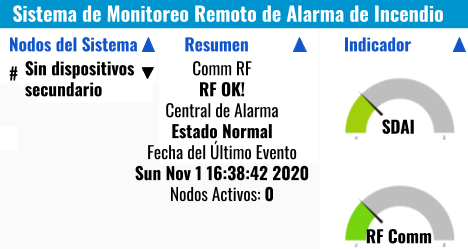
\includegraphics[scale=.55]{./Figures/Capitulo4/Figura_M.png}
	\caption{Interfaz web desarrollada para monitoreo del sistema utilizando la plataforma Node-RED.}
	\label{fig:figura_m}
\end{figure}

\subsubsection{Aplicación Android}
Aplicación móvil para dispositivos Android, conectada a la plataforma de Firebase para el monitoreo del sistema desde cualquier ubicación con conexión a Internet. En la figura \ref{fig:figura_n} se muestra una captura de pantalla de la interfaz.

\begin{figure}[ht]
	\centering
	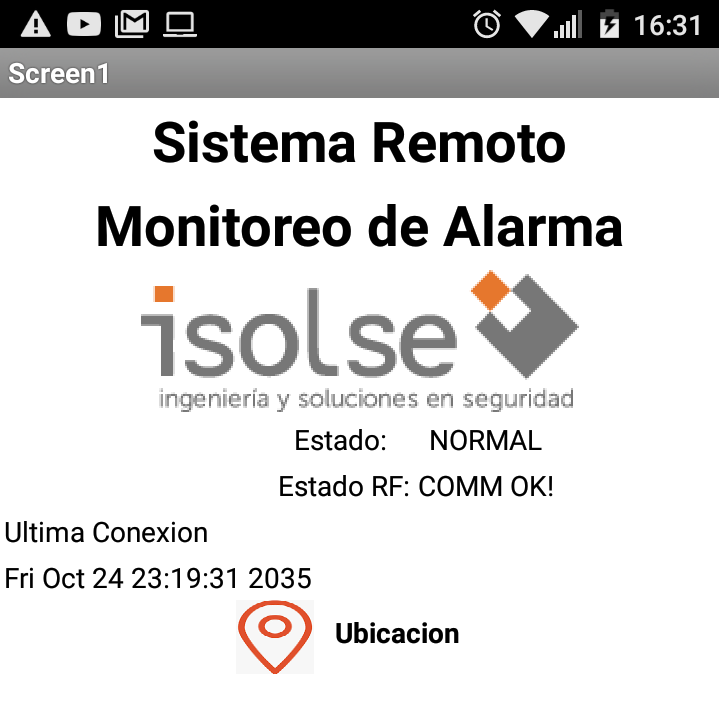
\includegraphics[scale=.35]{./Figures/Capitulo4/Figura_N.png}
	\caption{Aplicación móvil desarrollada con la plataforma MIT App Inventor, para visualización de datos cargados en el servidor web de Firebase.}
	\label{fig:figura_n}
\end{figure}

\subsubsection{Histórico de eventos como base de datos}
El registro de esta funcionalidad permite al sistema registrar de forma ordenada los eventos y otorga la posibilidad de analizar el histórico del sistema con el uso del lenguaje SQL. La figura \ref{fig:figura_p} corresponde a un ejemplo de histórico de eventos registrados a partir de una base de datos generada.

\break

\begin{figure}[ht]

	\centering
	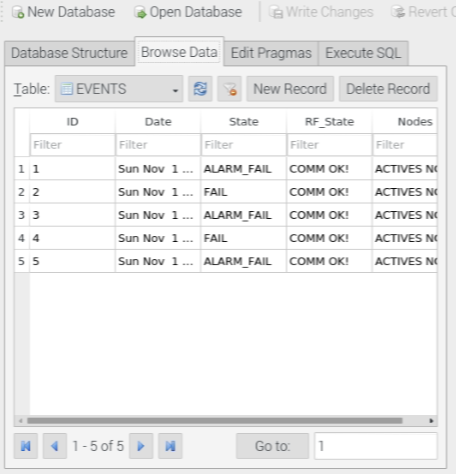
\includegraphics[scale=.45]{./Figures/Capitulo4/Figura_P.png}
	\caption{Ejemplo de histórico de eventos registrados en la base de datos.}
	\label{fig:figura_p}
\end{figure}

\subsubsection{Estado de red de dispositivos en base de datos}
Registro de nodos conectados al sistema en bases de datos --similar a la base de datos de registro de eventos--. Se incluye una base de datos con el registro de los nodos conectados, su estado actual y si se encuentran comunicándose correctamente con el dispositivo primario o no. La figura \ref{fig:figura_o}  muestra un ejemplo de la base de datos generada a partir de una red de dispositivos inalámbricos.


\begin{figure}[ht]
	\centering
	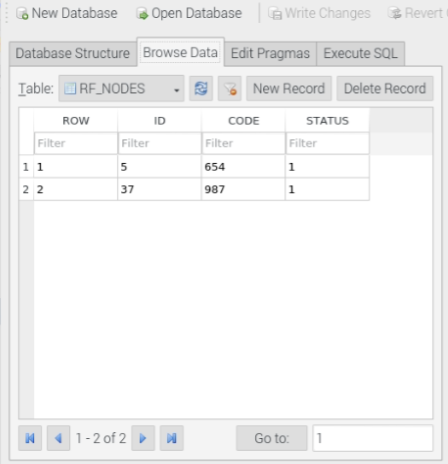
\includegraphics[scale=.45]{./Figures/Capitulo4/Figura_O.png}
	\caption{Ejemplo de la base de datos generada de una red de dispositivos inalámbricos.}
	\label{fig:figura_o}
\end{figure}

\break

\subsubsection{Implementación de \textit{Logging} }
Se hace uso de la biblioteca \textit{syslog} para facilitar el análisis en caso de fallas, registro de tareas de mantenimiento del sistema y uso como herramienta de desarrollo para futuros proyectos. Una vista del \textit{syslog} del sistema en funcionamiento se puede apreciar en la figura \ref{fig:figura_q}.


\begin{figure}[ht]
	\centering
	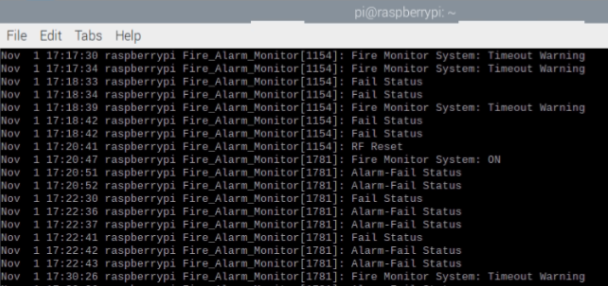
\includegraphics[scale=.65]{./Figures/Capitulo4/Figura_Q.png}
	\caption{Vista del archivo \textit{syslog} y los mensajes registrados por sistema de monitoreo.}
	\label{fig:figura_q}
\end{figure}

 
% Chapter Template

\chapter{Conclusiones} % Main chapter title

\label{Chapter5} % Change X to a consecutive number; for referencing this chapter elsewhere, use \ref{ChapterX}


%----------------------------------------------------------------------------------------

%----------------------------------------------------------------------------------------
%	SECTION 1
%----------------------------------------------------------------------------------------

\section{Conclusiones generales }

El trabajo finaliza con el desarrollo de un sistema de monitoreo remoto, compatible con sistemas de detección que funcionen con contactos secos programables. Además cuenta con la capacidad de establecer comunicación inalámbrica con diferentes dispositivos, en una estructura de red de nodos repetidores. Cada nodo ejecuta un protocolo de recuperación ante pérdidas de comunicación, que les permite restaurarse de forma automática ante diferentes eventos de falla, lo que evita en la gran mayoría de las ocasiones el traslado de personal técnico al lugar de la instalación. 

Este sistema fue puesto a prueba en obra para validar su correcto funcionamiento. Se utilizaron dispositivos con acceso web y se comprobó que el usuario pudiese visualizar el estado actual  de su sistema de seguridad de forma remota. 

Se resaltan las prácticas que fueron clave para cada etapa del proyecto:

\begin{itemize}
\item Planificación: aunque esta no se ejecutó según lo planteado originalmente, se considera una herramienta indispensable, ya que permite monitorear el progreso de las diferentes actividades que  integran el proyecto, así como identificar  retrasos  y/o  tareas que requieren mayor dedicación. Esto posibilita tomar las acciones necesarias en el tiempo adecuado para cumplir con los objetivos planteados.
\item Diseño: utilizar un patrón de diseño, combinado con una estrategia de desarrollo de software modularizado, permitió generar una estructura de código enfocado principalmente en escalabilidad. Este diseño evolucionó en una metodología de desarrollo, fundamentado en la elaboración de pequeños bloques funcionales probados con elementos de  \textit{testing}. Esto facilitó la inclusión de los conocimientos adquiridos a lo largo de la carrera de forma organizada.  
\item Software: a partir de las experiencias previas con sistemas operativos, fue posible realizar dos dispositivos funcionales, basados en sistemas operativos diferentes. El dispositivo primario aprovecha la gestión de un sistema operativo de propósito general para establecer una interfaz web bidireccional; asimismo el dispositivo secundario utiliza un sistema operativo cooperativo, que brinda compatibilidad con diferentes microcontroladores y a la vez escalabilidad al proyecto.   
\item Hardware: La fabricación de un dispositivo prototipo complementa la metodología de desarrollo de software explicada anteriormente, que genera una plataforma de prueba que permitió la elaboración de un sistema de pruebas continuas a medida que el sistema se iba concretando. Un aporte invaluable para el trabajo fueron los conocimientos adquiridos en el curso de diseño de circuitos impresos, donde se realizaron cambios al diseño original, que se ven reflejados en mejoras en las características de robustez, manufacturabilidad, detección de fallas y la generación documentación adecuada para el mantenimiento y evolución del proyecto. 
\end{itemize}


%----------------------------------------------------------------------------------------
%	SECTION 2
%----------------------------------------------------------------------------------------
\section{Próximos pasos}

El sistema actual cumple con los requerimientos planteados inicialmente. Sin embargo, durante su desarrollo surgieron puntos de mejora y trabajos a desarrollar, entre los cuales se resaltan los siguientes:

\begin{itemize}
\item Aprovechar la conectividad WiFi del dispositivo secundario, en función de establecer una vía alterna para la carga del estado del sistema en el servidor web, en caso de fallas en el dispositivo primario.
\item Desarrollo de una interfaz web personalizada, que complemente los avances realizados en la plataforma Node-RED. 
\item Diseño de un tercer dispositivo que funcione como nodo repetidor, que prescinda de funcionalidades adquisición de información y se enfoque en extender el alcance de la comunicación por radiofrecuencia.    
\item Implementación de un servidor que regule el acceso de los usuarios, que además permita visualizar la información desde cualquier punto con conectividad a Internet.
\end{itemize}

El sistema actual se basa en el monitoreo de contactos secos programables, con el objetivo de mantener compatibilidad con diferentes marcas comerciales. A la vez existen segmentos del mercado con requerimientos más exigentes. Algunos posibles proyectos son:


\begin{itemize}
\item Hacer uso del puerto de conexión de impresoras de algunas marcas comerciales de centrales de alarma de incendio, para obtener un mayor detalle de los eventos que ocurren en la instalación.
\item Diseñar una interfaz gráfica que se adecue a cada obra, que facilite al usuario la documentación de la instalación, tal como información de los equipos instalados, instrucciones ante diferentes eventos, planos con el estado de real de los dispositivos, datos históricos, próximos mantenimientos, etc.
\end{itemize}

Un aporte significativo que se espera poder alcanzar con esta serie de proyectos consiste en establecer un sistema con la robustez y confiabilidad suficiente para instaurar un vínculo con personal capacitado. Ello puede favorecer a generar una respuesta temprana ante situaciones de incendio, que disminuya los daños ocasionados y salvaguarde de manera eficaz la vida de las personas en situaciones de emergencia. 
 

%----------------------------------------------------------------------------------------
%	CONTENIDO DE LA MEMORIA  - APÉNDICES
%----------------------------------------------------------------------------------------

\appendix % indicativo para indicarle a LaTeX los siguientes "capítulos" son apéndices

% Incluir los apéndices de la memoria como archivos separadas desde la carpeta Appendices
% Descomentar las líneas a medida que se escriben los apéndices

%% Appendix A

\chapter{Appendix Title Here} % Main appendix title

\label{AppendixA} % For referencing this appendix elsewhere, use \ref{AppendixA}

Write your Appendix content here.
%\include{Appendices/AppendixB}
%\include{Appendices/AppendixC}

%----------------------------------------------------------------------------------------
%	BIBLIOGRAPHY
%----------------------------------------------------------------------------------------

\Urlmuskip=0mu plus 1mu\relax
\raggedright
\printbibliography[heading=bibintoc]

%----------------------------------------------------------------------------------------

\end{document}  
